\documentclass[11pt]{report}
\usepackage{graphicx}
\usepackage{index}
\usepackage{varioref}
\usepackage{amsmath}
\usepackage{multirow}
\usepackage{theorem} % for examples
\usepackage{alltt}
\usepackage{ulem}
\usepackage{epic,eepic}
\usepackage{boxedminipage}
\usepackage{fancybox}
\usepackage[square]{natbib}
\usepackage{epsfig}
%\usepackage{subfig}
\usepackage{subfigure}
\usepackage{booktabs}

\usepackage[encapsulated]{CJK}
\usepackage{ucs}
\usepackage[utf8x]{inputenc}
% use one of bsmi(trad Chinese), gbsn(simp Chinese), min(Japanese), mj(Korean); see:
% /usr/share/texmf-dist/tex/latex/cjk/texinput/UTF8/*.fd
\newcommand{\cntext}[1]{\begin{CJK}{UTF8}{gbsn}#1\end{CJK}}


\oddsidemargin 0mm
\evensidemargin 5mm
\topmargin -20mm
\textheight 240mm
\textwidth 160mm



\newcommand{\bold}{\it}
\renewcommand{\emph}{\it}

\makeindex
\theoremstyle{plain}

\newcommand{\nt}[2]{\textrm{#1}_{\framebox[5pt]{\scriptsize #2}}}
\newcommand{\ind}[1]{{\fboxsep1pt\raisebox{-.5ex}{\fbox{{\tiny #1}}}}}

\begin{document}
\title{\vspace{-15mm}\LARGE {\bf Final Report}\\[2mm]
of the\\[2mm]
2010 Language Engineering Workshop\\[15mm]
{\huge \bf Models for\\
Synchronous Grammar Induction\\[2mm]
{\tt \Large http://www.clsp.jhu.edu/workshops/ws10/groups/msgismt/}\\[15mm]
Johns Hopkins University\\[2mm]
Center for Speech and Language Processing}}
\author{\large Phil Blunsom,
Chris Callison-Burch,
Trevor Cohn,
Chris Dyer,
Adam Lopez,\\
\large
Jonathan Graehl,
Jonathan Weese,
Jan Botha,
Vladimir Eidelman,
ThuyLinh Nguyen,
Ziyuan Wang, \\
\large Olivia Buzek, Desai Chen}
\normalsize

\maketitle

\section*{Abstract}
The last decade of research in Statistical Machine Translation (SMT) has seen rapid progress. The most successful methods have been based on synchronous context free grammars (SCFGs), which encode translational equivalences and license reordering between tokens in the source and target languages. Yet, while closely related language pairs can be translated with a high degree of precision now, the result for distant pairs is far from acceptable. In theory, however, the ``right'' SCFG is capable of handling most, if not all, structurally divergent language pairs. The 2010 Language Engineering Workshop {\emph Models of Synchronous Grammar Induction for SMT} had the goal to focus on the crucial practical aspects of acquiring such SCFGs from bilingual text. We started with existing algorithms for inducing unlabeled SCFGs (e.g. the popular Hiero model) and then used state-of-the-art unsupervised learning methods to refine the syntactic constituents used in the translation rules of the grammar.

\phantom{.}


\newpage
\section*{Acknowledgments}
The participants at the workshop would like to thank everybody at Johns Hopkins University who made the summer workshop such a memorable --- and in our view very successful --- event. The JHU Summer Workshop is a great venue to bring together researchers from various backgrounds and focus their minds on a problem, leading to intense collaboration that would not have been possible otherwise.

We especially would like to thank Fred Jelinek for heading the Summer School effort and Desir\'ee Cleves for her superhuman ability to keep things running smoothly.

\phantom{.}

\newpage
\section*{Team Members}

\begin{itemize}
\item Phil Blunsom, Team Leader, University of Oxford
\item Chris Callison-Burch, Senior Researcher, Johns Hopkins University
\item Trevor Cohn, Senior Researcher, University of Sheffield
\item Chris Dyer, Senior Researcher, Carnegie Mellon University
\item Adam Lopez, Senior Researcher, University of Edinburgh
\item Jonathan Graehl, Senior Researcher, Information Sciences Institute, USC
\item Jan Botha, Graduate Student, University of Oxford
\item Vladimir Eidelman, Graduate Student, University of Maryland
\item Thuylinh Nguyen, Graduate Student, Carnegie Mellon University
\item Jonathan Weese, Graduate Student, Johns Hopkins University
\item Ziyuan Wang, Graduate Student, Johns Hopkins University
\item Olivia Buzek, Undergraduate Student, University of Maryland
\item Desai Chen, Undergraduate Student, Carnegie Mellon University
\end{itemize}
\tableofcontents


\chapter{Introduction}

Automatically generating high quality translations for foreign texts remains a central challenge for natural language processing research.
Recent advances in statistical machine translation (SMT) has enabled these technologies to move out of research labs an become viable commercial products and useful online tools. \footnote{e.g., translate.google.com, www.systran.co.uk, www.languageweaver.com} 
However these successes have not been uniform; 
current state-of-the-art translation output varies markedly in quality depending on the languages being translated. 
Those language pairs that are closely related language pairs (e.g., English and French) can be translated with high quality, while for distant pairs (e.g., English and Chinese) the result tends to be much lower quality. 
It is tempting to argue that SMT's current limitations can be overcome simply by increasing the amount of data on which the systems are trained. 
However, large scale evaluation campaigns for Chinese~$\rightarrow$~English translation, such as the DARPA GALE program, have not yielded high quality translation despite providing hundreds of millions of words worth of training data. 

\begin{figure}[t]
  \centering 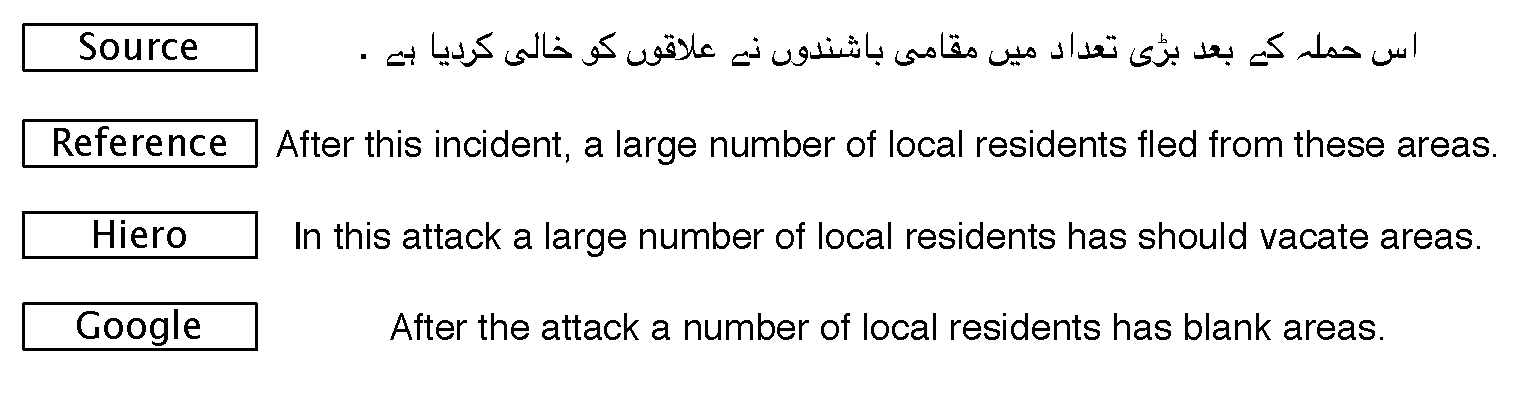
\includegraphics[scale=0.55]{urdu_example_translation.pdf}
\caption{An example Urdu $\rightarrow$ English translation show outputs from both a state-of-the-art Hiero translation model, and Google's translation service.}
\label{fig:intro_urdu_example}
\end{figure}
Figure \ref{fig:intro_urdu_example} shows the current state-of-the-art for translating an Urdu sentence into English.
While a considerable portion of the content of the input Urdu sentence is translated, the end result is still far from being acceptable for an end user. 
%\begin{figure}
%  \centering \includegraphics[scale=1.3]{intro_slides/WhoWroteThisLetter.pdf}
%\caption{The level of structural divergence varies depending on the language pair in question.}
%\label{fig:intro_translation_divergence}
%\end{figure}
Many of the issues faced by SMT systems can be attributed to structural divergence between the languages being translated.
While many researchers are tackling these issues, most proposed solutions are limited by focusing on more expressive models of translation rather than addressing the issue of how, and what, translation units are learnt a priori.


\begin{table}[t]
\centering
  \begin{tabular}{l|rr}
    \hline
    Language & Words &  Domain \\ \hline
    English & 4.5M& Financial news \\
    Chinese & 0.5M & Broadcasting news \\ 
    Arabic &  300K (1M planned)  &  News  \\
    Korean & 54K  & Military \\ \hline
  \end{tabular}
\caption{Major treebanks: data size and domain.}
\label{tab:intro_treebanks}
\end{table}
%\begin{figure}
%  \centering 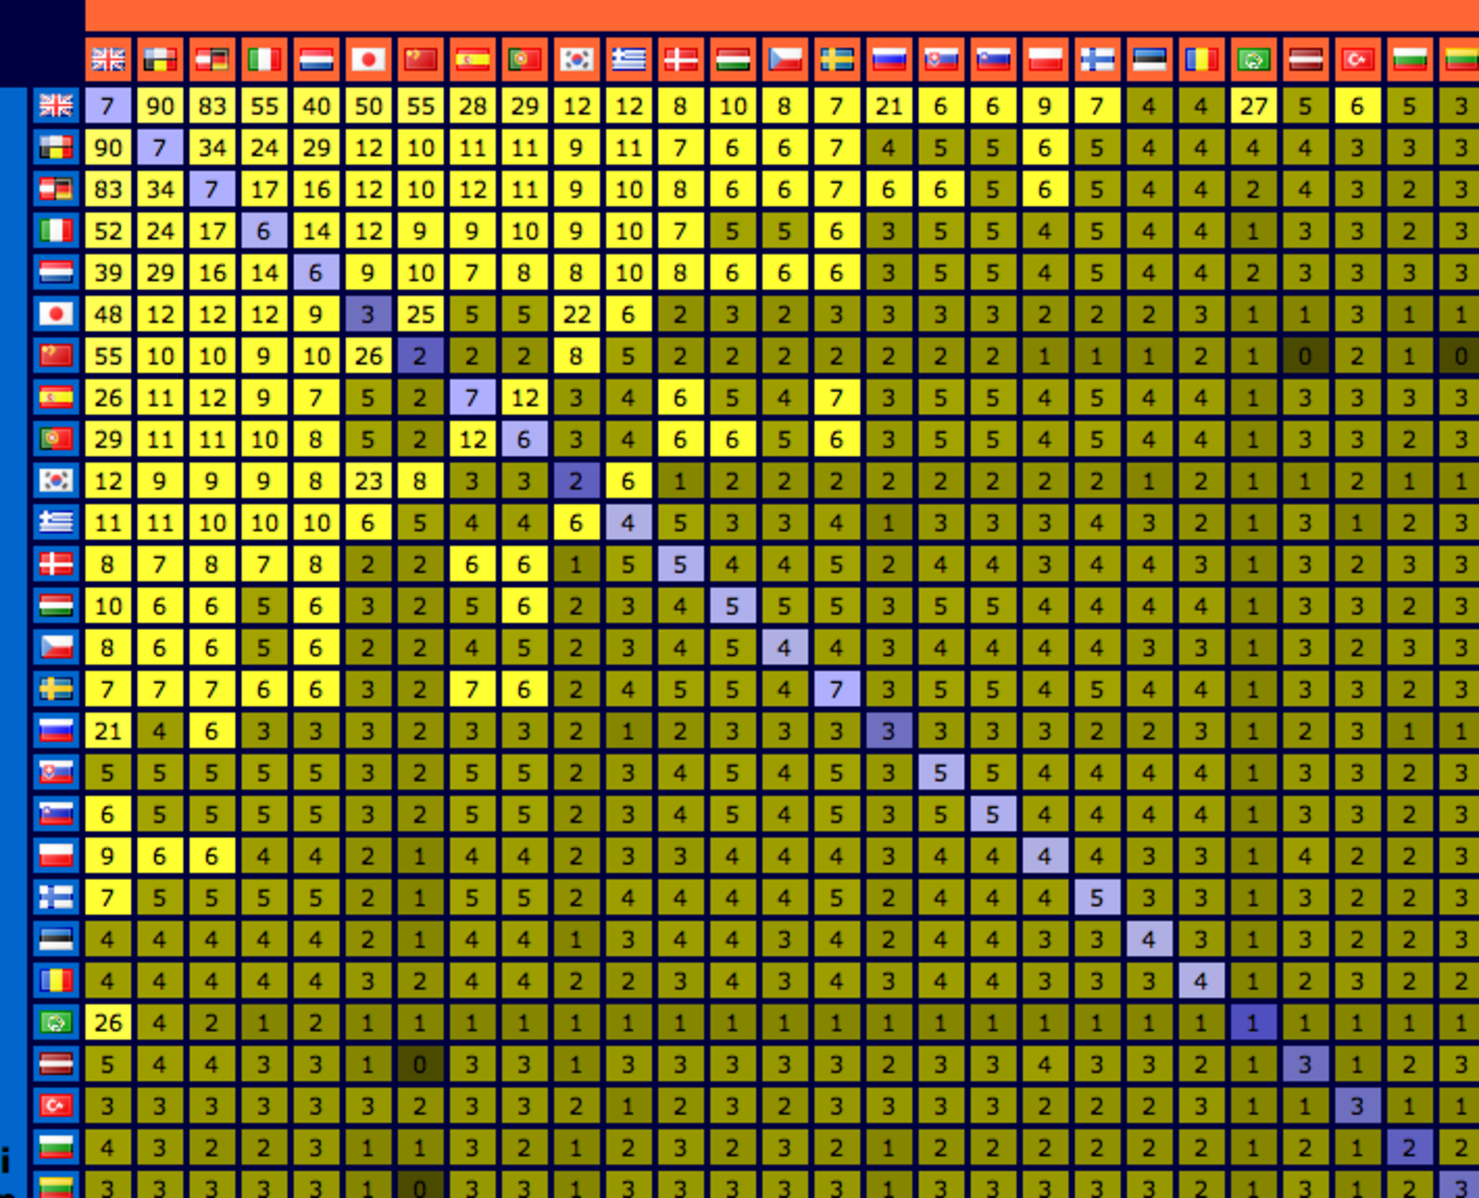
\includegraphics[scale=0.3]{intro_slides/resource_matrix.pdf}
%\caption{A matrix of the number of parrallel words available for various language pairs.}
%\label{fig:intro_parallel_words_matrix}
%\end{figure}

\begin{figure}[t]
  \centering
  \subfigure{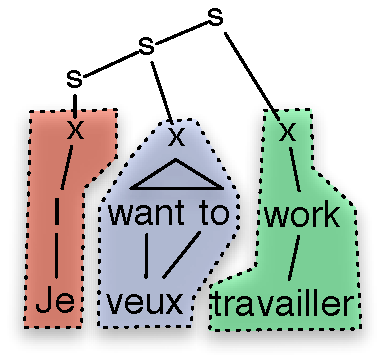
\includegraphics[scale=0.5]{intro_slides/JeVeuxTravailler-Hiero.pdf}}
  \subfigure{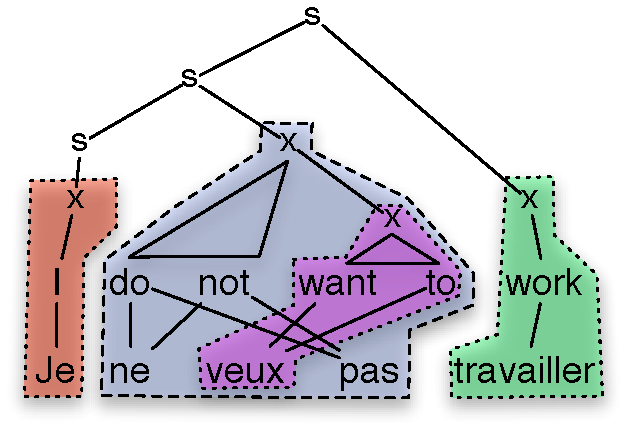
\includegraphics[scale=0.5]{intro_slides/JeNeVeuxPasTravailler-Hiero.pdf}}
\caption{Example derivations using the Hiero grammar extraction heuristics \cite{chiang07hierarchical}.}
\label{fig:intro_hiero}
\end{figure}

\begin{figure}[t]
  \centering
  \subfigure{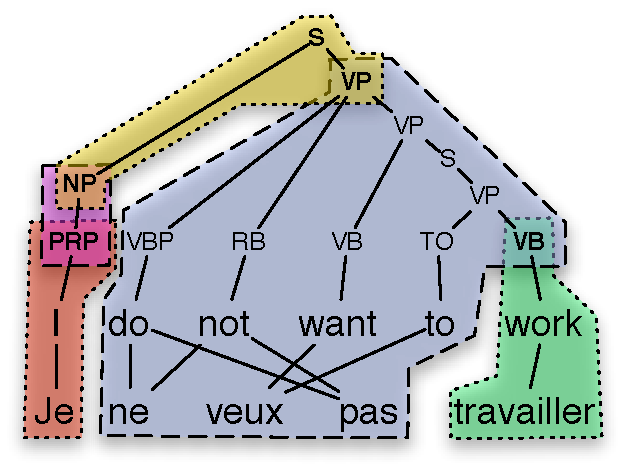
\includegraphics[scale=0.5]{intro_slides/JeNeVeuxPasTravailler-tsg.pdf}}
  \subfigure{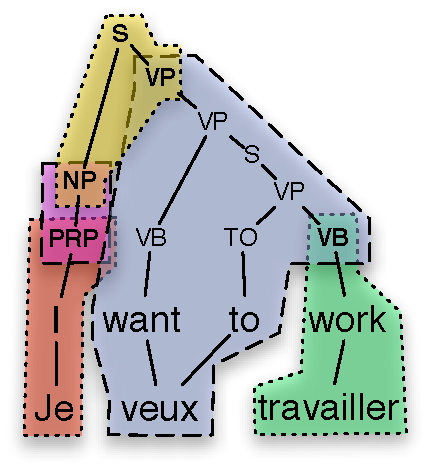
\includegraphics[scale=0.5]{intro_slides/JeVeuxTravailler-tsg.pdf}}
\caption{Example derivations for a Tree Substitution Grammar derived from a parallel corpus parsed with a supervised parser.}
\label{fig:intro_tsg}
\end{figure}

Models which have been most successful for translating between structurally divergent language pairs have been based on synchronous grammars. 
A critical component of these translation models is their {\emph grammar} which encodes translational equivalence and licenses reordering between tokens in the source and target languages. 
There is considerable scope for improving beyond current techniques for automatically acquiring synchronous grammars from bilingual corpora, which seek to find either extremely simple grammars with only one non-terminal or else rely on treebank-trained parsers.
The advantage of using a simple grammar is that no extra annotated linguistic resources are required beyond the parallel corpus.
However these simple grammars are incapable of representing the substitutability of a constituent.
Figure \ref{fig:intro_hiero} displays a synchronous derivation in such a simple grammar.
Richer grammars induced from a parallel corpus annotated with syntax trees overcome the limitations of the simple grammars and provide a far more powerful representation of language structure. 
Figure \ref{fig:intro_tsg} shows a synchronous derivation in for a grammar extracted parallel corpus parsed on the English side.
The limitation of this approach is that the reliance on supervised parses restricts the systems' portability to new target languages (effectively limiting us to translating into/out of English) while enforcing a restrictive notion of linguistic constituency. 
Figure \ref{fig:intro_parallel_words_matrix} shows the number of words in the treebanks available for the most well resourced languages. 
As the performance of supervised parsers is heavily dependent on the amount of training data available, clearly we can expect poorer results when building translation models based upon then for languages other than English.
A further, but more subtle, limitation of these models is the assumption that the particular brand of linguistic structure assigned by a parser (usually a form of phrase structure grammar learnt from the Penn. Treebank) is predominantly isomorphic to that of the input language; an assumption which is rarely true for distantly related language pairs, or even closely related ones.



Clearly there is a need for research into the unsupervised induction of synchronous grammar based translation models.
Previous research has focussed on structured learning approaches requiring costly global inference over translation pair derivations, limiting the ability of these models to be scaled to large datasets \cite{blunsom09bscfg}.
In this workshop we adopted a pragmatic approach of embracing existing algorithms for inducing unlabelled SCFGs (e.g. the popular Hiero model \cite{chiang07hierarchical}), and then used state-of-the-art probabilistic models to independently learn syntactic classes for translation rules in the grammar.
We structured the workshop into three parallel but interdependent streams:

\begin{figure}
  \centering
  \subfigure{\includegraphics[scale=0.5]{intro_slides/JeNeVeuxPasTravailler-hiero-labelled.pdf}}
\caption{Example derivation using the Hiero grammar extraction heuristics where non-terminals have been clustered into unsupervised syntactic categories denoted by $X?$.}
\label{fig:intro_labelled_hiero}
\end{figure}


\paragraph{1) Unsupervised induction of labelled SCFGs}
Inspired by work in monolingual PCFG learning, we have investigated generative models which describe the production of phrase translations in terms of sequences of tokens (or word classes) and their observed contexts.
We simplify the grammar induction problem to first clustering monolingual phrases based upon their distribution over contexts (preceding and following words), and then intersecting these labelled phrases with the Hiero \cite{chiang07hierarchical} SCFG rule extraction heuristics. 
The end result are grammars that produce derivations like that in Figure \ref{fig:intro_labelled_hiero}, where the labels are the unsupervised clusters induced by our context based induction algorithm.

We explored two approaches to the clustering of phrases.
The first was inspired by research in Topic Modelling, in particular Latent Dirichlet Allocation (LDA).
We formulated a model in which each phrase type maintains a distribution over labels, and each context a phrase appears in is generated by first choosing a label, and then generating the context from this labels distribution over contexts.
We extended the basic LDA model to incorporate hierarchical Pitman Yor distributions on the two generating components of the model.
In the second approach we optimised the same model as describe above, but in instead of using non-parametric Bayesian approach to encouraging sparsity in the model, we used the direct Posterior Regularisation technique of \cite{someone}. 

The labelled SCFGs produced by these algorithms generate a subset of the translations licensed by the original Hiero grammars.
While we hope that this restriction guides the model to more acceptable translations, with the inevitable noise present in all automatically induced translation models it is advantageous to allow our models to degrade gracefully to less restrictive grammars.
As such we also explored hierarchical cascades of grammars, each of which was induced with a different number of labels, allowing the translation model to switch between these while incurring a penalty for doing so.

This work on inducing labels for SCFGs formed the core component of the workshop and the base for the following work exploiting these labellings. 
By the conclusion of the workshop we were able to demonstrate that applying these induction techniques leads to improved translations for both Chinese$\rightarrow$English and Urdu$\rightarrow$ translation systems.
Chapter \ref{chap:grammar_induction} describes this work.

\paragraph{2) Decoding with labelled SCFGs}
The second major component of the workshop involved the investigation of improved decoding algorithms for the type of labelled SCFG produced by our induction methods.
Decoding complexity scales quadratically with the number of labels in the grammar.
As such inducing grammars with more than one label significantly increases the time and resources required for decoding.
We explored a number of avenues for reducing this computational burden, including the early pruning items from the search space before language model integration, and coarse-to-fine techniques in which decoding is performed with grammars with progressively more labels and pruning at each step.
We were able to show that each of these techniques could lead to faster decoding without compromising translations performance.
Chapter \ref{chap:decoding} describes this work.

\paragraph{3) Discriminative training labelled SCFG translation models}
The third stream of the workshop focussed on implementing discriminative training algorithms for the labelled SCFG translation models produced by our unsupervised grammar induction algorithms.
Though the existing MERT \cite{och02mert} training algorithm is directly applicable to these grammars, it doesn't allow us to optimise models with large numbers of fine grained features extracted from the labels we've induced.
In order to maximise the benefit from our induced grammars we explored and implemented discriminative training algorithms capable of handling thousands, rather than tens, of features.
The algorithms we explored were Maximum Expected Bleu \cite{smith,li} and MIRA \cite{chiang}.
Chapter \ref{chap:training} describes this work.

The remainder of this introductory chapter provides a formal definition of SCFGs and describes the language pairs that we experimented with.

\section{Synchronous context free grammar} \label{sec:scfg}

A synchronous context free grammar (SCFG, \cite{lewis68scfg}) generalizes context-free grammars to generate strings concurrently in two (or more) languages. A string pair is generated by applying a series of paired rewrite rules of the form, $X \rightarrow \langle \mathbf{e}, \mathbf{f}, \mathbf{a} \rangle$, where $X$ is a non-terminal, $\mathbf{e}$ and $\mathbf{f}$ are strings of terminals and non-terminals and $\mathbf{a}$ specifies a one-to-one alignment between non-terminals in $\mathbf{e}$ and $\mathbf{f}$.
In the context of SMT, by assigning the source and target languages to the respective sides of a probabilistic SCFG it is possible to describe translation as the process of parsing the source sentence, which induces a parallel tree structure and translation in the target language \cite{chiang07hierarchical}.  
Terminal are rewritten as pairs of strings of terminal symbols in the source and target languages.  Additionally, one side of a terminal expansion may be the special symbol $\epsilon$, which indicates a null alignment which permits arbitrary insertions and deletions.
Figure \ref{fig:scfg} shows an example derivation for Japanese to English translation using an SCFG.

\begin{figure}Grammar fragment:
\begin{eqnarray*}
\label{rule:discont}X & \rightarrow & \langle \nt{X}{1}\ \nt{X}{2}\ \nt{X}{3},\ \nt{X}{1}\ \nt{X}{3}\ \nt{X}{2} \rangle  \\
X & \rightarrow & \langle \textrm{\emph{John-ga}},\ \textrm{\emph{John}} \rangle  \\
X & \rightarrow & \langle \textrm{\emph{ringo-o}},\ \textrm{\emph{an apple}} \rangle  \\
X & \rightarrow & \langle \textrm{\emph{tabeta}},\ \textrm{\emph{ate}} \rangle
\end{eqnarray*}
Sample derivation:
\begin{eqnarray*}
\label{derivationt}
& &\langle \nt{S}{1},\nt{S}{1} \rangle \Rightarrow \langle \nt{X}{2},\ \nt{X}{2} \rangle \\
 & \Rightarrow&  \langle \nt{X}{3}\ \nt{X}{4}\ \nt{X}{5},\ \nt{X}{3}\ \nt{X}{5}\ \nt{X}{4} \rangle  \\
 & \Rightarrow &\langle \textrm{\emph{John-ga}}\ \nt{X}{4}\ \nt{X}{5},\ \textrm{\emph{John}}\ \nt{X}{5}\ \nt{X}{4} \rangle \\
 & \Rightarrow &\langle \textrm{\emph{John-ga}}\ \textrm{\emph{ringo-o}}\ \nt{X}{5},\ \textrm{\emph{John}}\ \nt{X}{5}\ \textrm{\emph{an apple}} \rangle \\
 & \Rightarrow &\langle \textrm{\emph{John-ga ringo-o tabeta}},\ \textrm{\emph{John ate an apple}} \rangle
\end{eqnarray*}
\caption{A fragment of an SCFG with a ternary non-terminal expansion and three terminal rules.}
\label{fig:scfg}
\end{figure}

The generative story is as follows. 
In the beginning was the grammar, in which we allow  two types of rules: {\emph non-terminal} and {\emph terminal} expansions. 
The former rewrites a non-terminal symbol as a string of two or three non-terminals along with an alignment $\mathbf{a}$, specifying the corresponding ordering of the child trees in the source and target language. 
Terminal expansion rewrite a non-terminal as a pair of terminal n-grams, where either but not both may be empty. 
Given a grammar, each sentence is generated as follows, starting with the distinguished root non-terminal, $S$. 
Rewrite each frontier non-terminal, $c$, using a rule chosen from our grammar expanding $c$. 
Repeat until there are no remaining frontier non-terminals. 
The sentences in both languages can then be read off the leaves, using the rules' alignments to find the right ordering. 




\chapter{Synchronous context free grammars} \label{sec:scfg}



\begin{figure}
\begin{center}
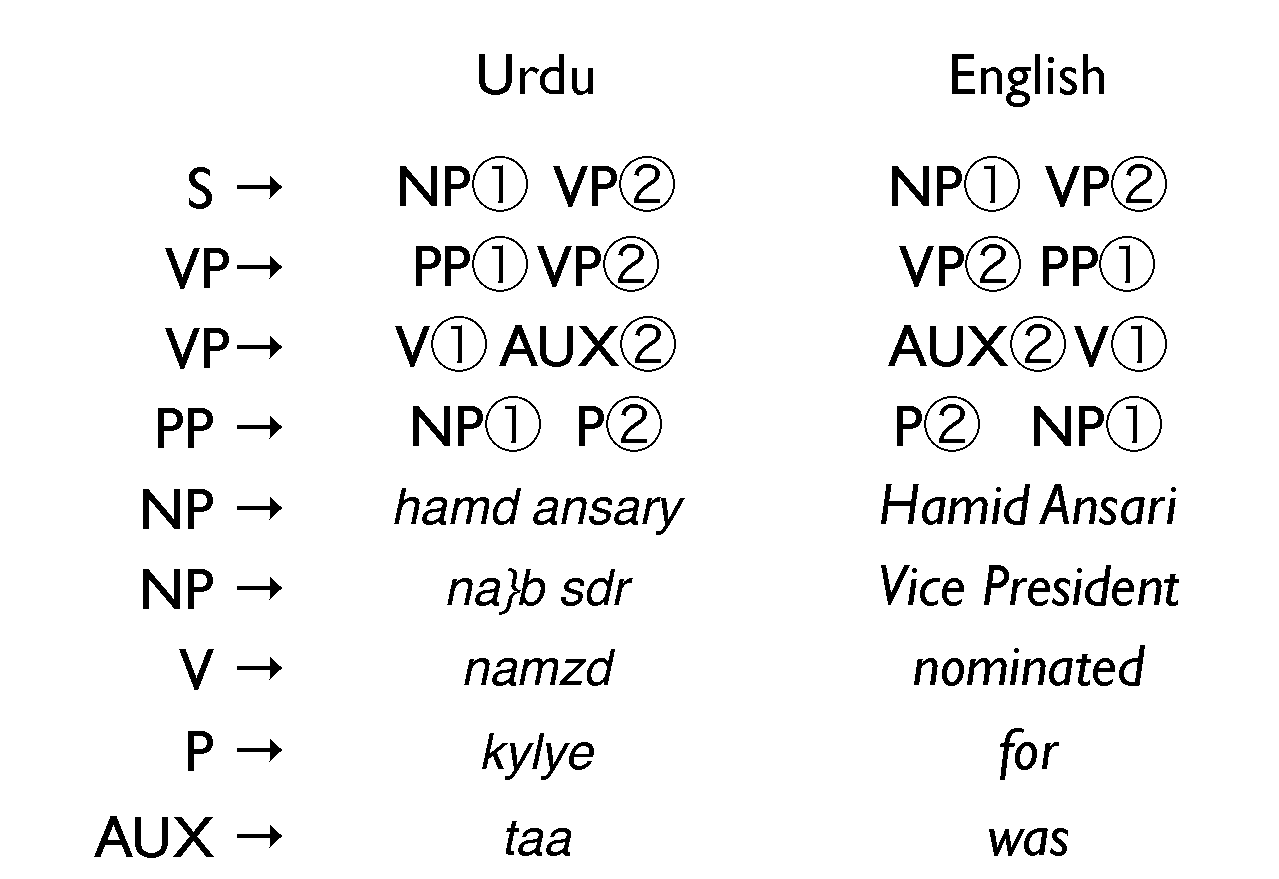
\includegraphics[width=.6\linewidth]{SCFGs/example-scfg}
\end{center}
\caption{A toy example that illustrates a SCFG that can translate (romanized) Urdu into English for one sentence.    }\label{toy-scfg} 
\end{figure}


\begin{figure}
\begin{tabular}{lll}
\multicolumn{3}{>{\columncolor[rgb]{0.95,0.95,0.75}}c}{The input is an Urdu sentence which is initially unanalyzed.}\\
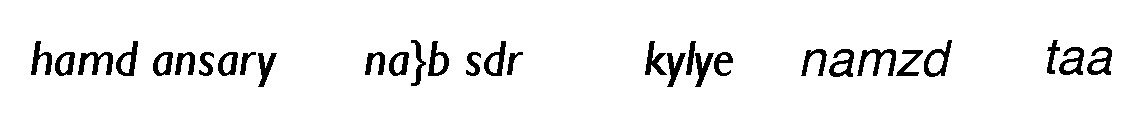
\includegraphics[width=.45\linewidth]{SCFGs/urdu-input} &  & 
\\ \hline
\multicolumn{3}{>{\columncolor[rgb]{0.95,0.95,0.75}}c}{Here all of the terminal symbols receive non-terminal labels.  The English words are in Urdu order.}\\
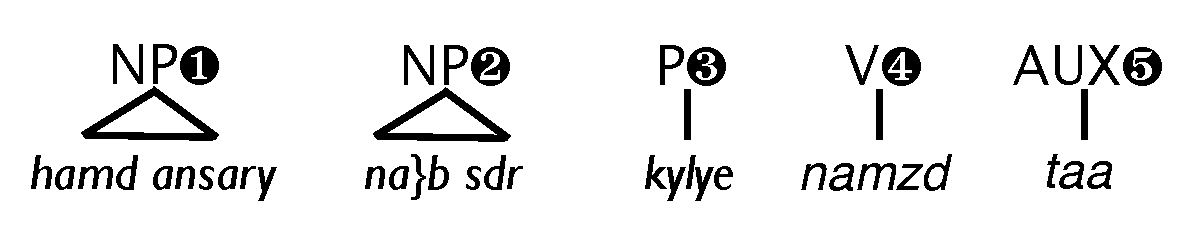
\includegraphics[width=.45\linewidth]{SCFGs/urdu-step0} & &
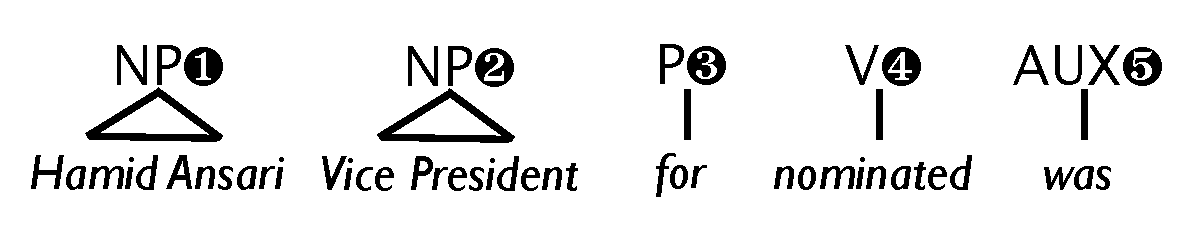
\includegraphics[width=.45\linewidth]{SCFGs/english-step0} \\ \hline
\multicolumn{3}{>{\columncolor[rgb]{0.95,0.95,0.75}}c}{The PP rule reorders the Urdu postpositional phrase to be a prepositional phrase on the English side.}\\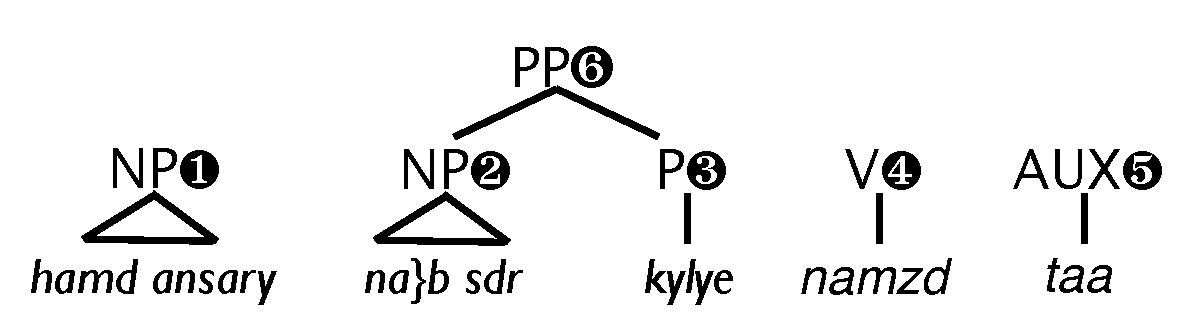
\includegraphics[width=.45\linewidth]{SCFGs/urdu-step1} & &
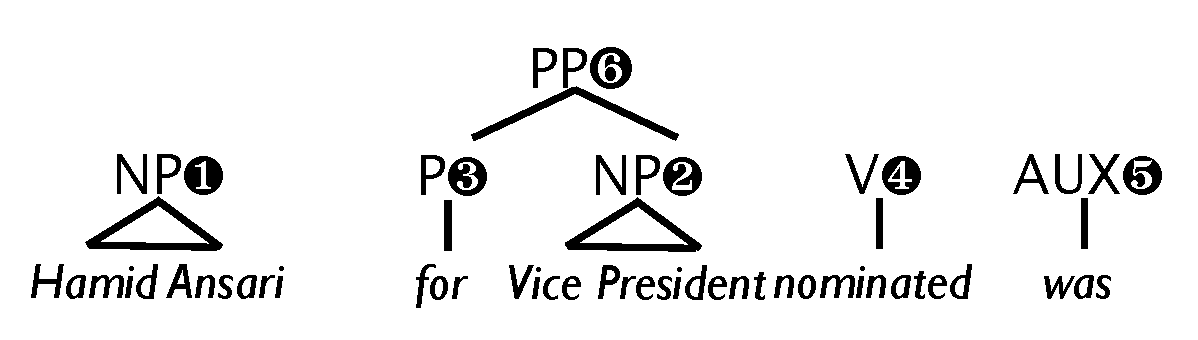
\includegraphics[width=.45\linewidth]{SCFGs/english-step1} \\ \hline\multicolumn{3}{>{\columncolor[rgb]{0.95,0.95,0.75}}c}{The English auxiliary verb and main verb get reordered with the application of the VP rule.}\\
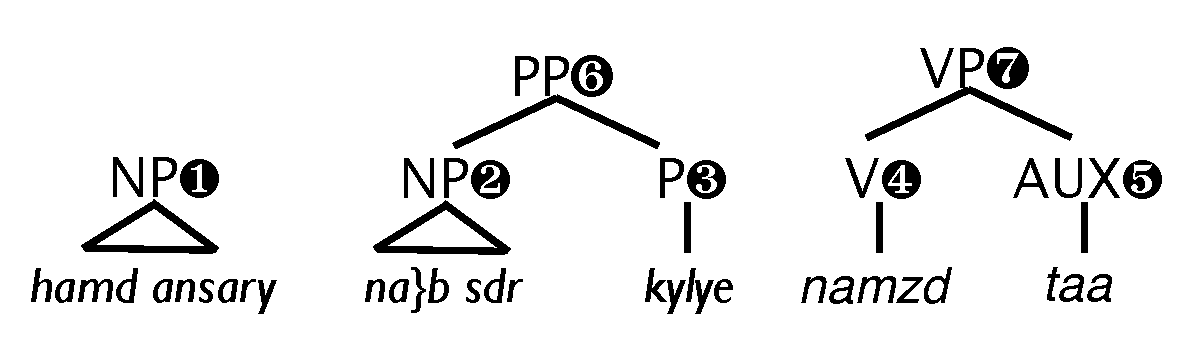
\includegraphics[width=.45\linewidth]{SCFGs/urdu-step2} & &
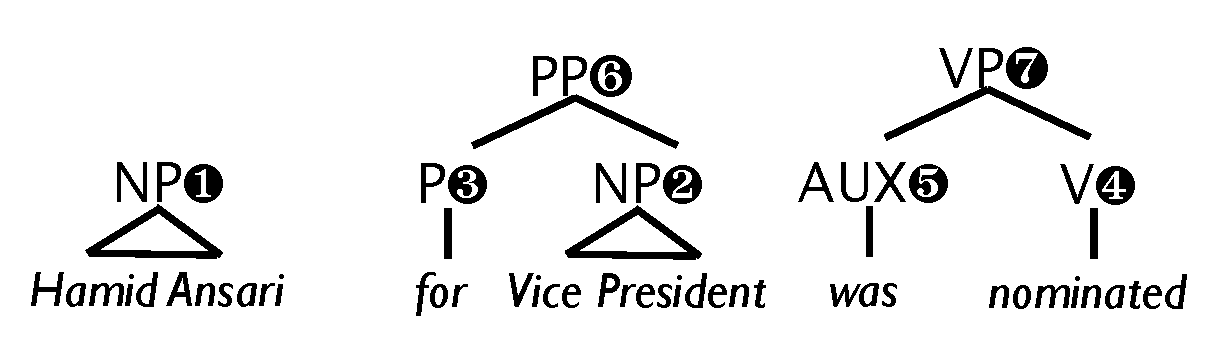
\includegraphics[width=.45\linewidth]{SCFGs/english-step2} \\ \hline 
\multicolumn{3}{>{\columncolor[rgb]{0.95,0.95,0.75}}c}{This VP rule moves the English verb from the Urdu verb-final position to its correct place before the PP.}\\
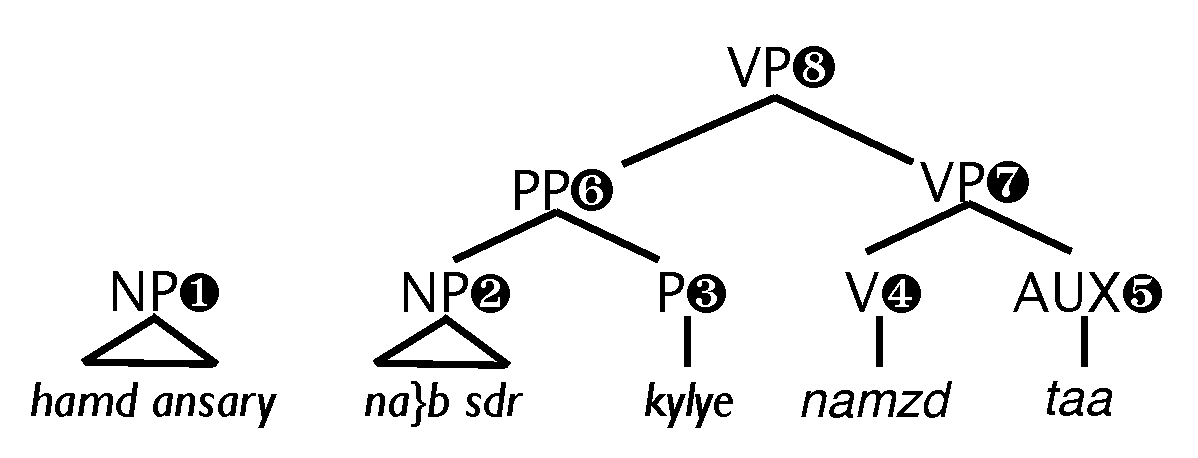
\includegraphics[width=.45\linewidth]{SCFGs/urdu-step3} &  & 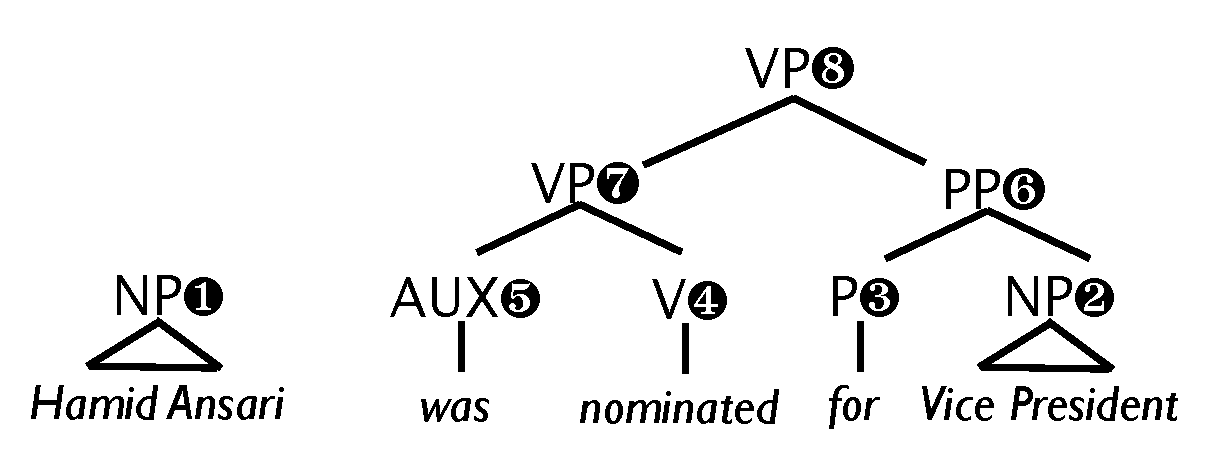
\includegraphics[width=.45\linewidth]{SCFGs/english-step3} \\ \hline
\multicolumn{3}{>{\columncolor[rgb]{0.95,0.95,0.75}}c}{Applying the S rule, means that we have a complete translation of the Urdu sentence.}\\
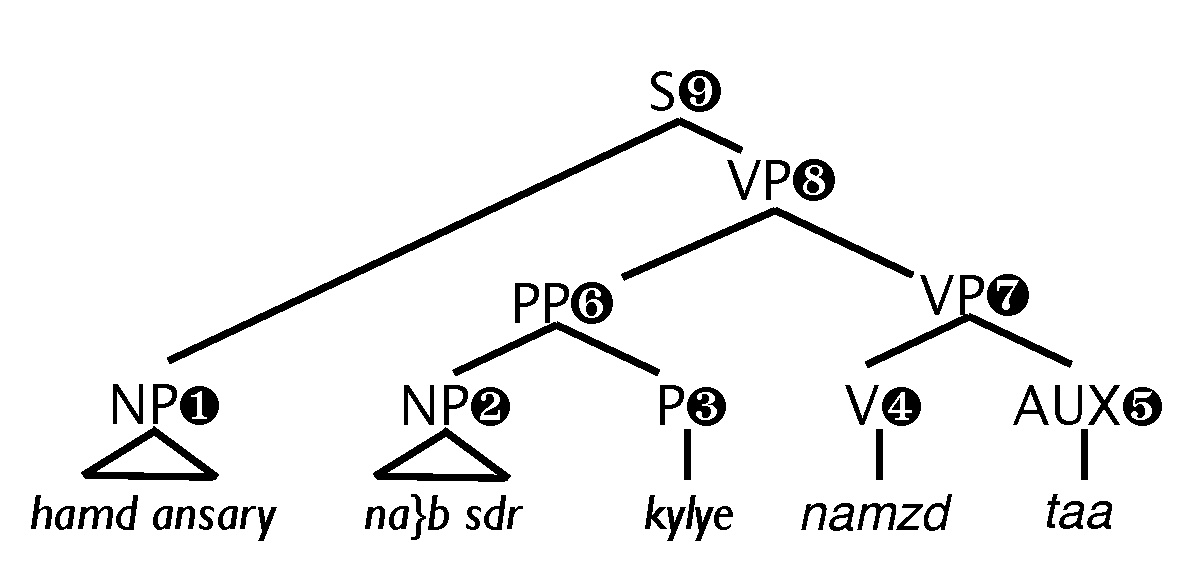
\includegraphics[width=.45\linewidth]{SCFGs/urdu-step4} &  & 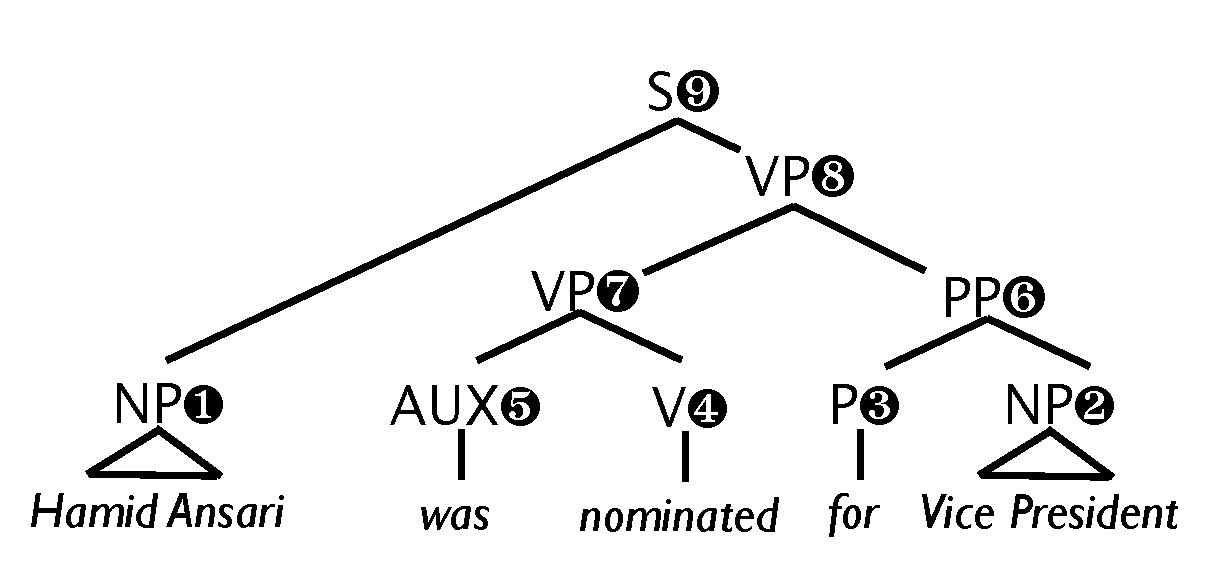
\includegraphics[width=.45\linewidth]{SCFGs/english-step4} 
\end{tabular}
\caption{Using SCFGs as the underlying formalism means that the process of translation is one of parsing.  This shows how an English sentence can be generated by parsing the Urdu sentence using the rules given in Figure \ref{toy-scfg}}\label{toy-scfg-parse} 
\end{figure}



The translation models used in this workshop are synchronous context free grammars (SCFGs).
SCFGs \cite{lewis68scfg}  generalize  context free grammars so they generate pairs of related strings.  
Because they generate pairs of strings they are useful for specifying the relationship between two languages, and can be used to describe translation and re-ordering.  
Probabilistic SCFGs can be formally defined as follows:
\begin{itemize}
\item T$_{S}$: a set of source-language terminal symbols
\item T$_{T}$: a set of target-language terminal symbols
\item N: a shared set of nonterminal symbols
\item A set of rules of the form  $\text{X} \rightarrow \langle \gamma, \alpha, \sim, w \rangle$
	\begin{itemize}
	\item X $\in$ N
	\item $\gamma$ is a sequence source terminals and non-terminals
	\item $\alpha$ is a sequence of target terminals and non-terminals
	\item $\sim$ is a one-to-one correspondence between the non-terminals in  $\gamma$  and $\alpha$
	\item $w$ is a weight or probability assigned to the rule
	\end{itemize}
\end{itemize}



A toy example of an SCFG is given in Figure \ref{toy-scfg}.  The nonterminal symbols, which are written in uppercase, are identical across the two right hand sides of the context free grammar rules, but can come in different orders. 
The process of translation is accomplished by parsing the source language input sentence and simultaneously generating the target language output sentence.  This
process is illustrated in Figure \ref{toy-scfg-parse}, which shows how parsing an  Urdu sentence generates an English translation using the toy example grammar.  The toy grammar and example parse omit the $w$ weights/probabilities assigned to the grammar rules.  In practice there are a huge number of alternative translations and derivations, and assigning probabilities allows us to choose the best translation according to the model, and to reduce the search space by expanding only the most promising partial translations. 

\subsection{Hiero: SCFGs with one non-terminal symbol}

The use of SCFGs for statistical machine translation was popularized by \citet{Chiang2005} with the introduction of the Hiero system.  Chiang's Hiero system extended the standard phrase-based approaches to statistical machine translation by allowing phrases that contain gaps.  Chiang described how these {\it hierarchical phrases} could be obtained by straightforwardly extending the standard methods \cite{Koehn2004,Koehn2003,Tillmann2003,Venugopal2003} for extracting phrase pairs from word-aligned sentence pairs.  Figure \ref{hiero-phrase-extraction} shows how a hierarchical phrase can be constructed by replacing two smaller phrase pairs with the nonterminals indexed $1$ and $2$.   These rules are written in the same format as the SCFG rules given in Figure \ref{toy-scfg}.  Although the Hiero rules are devoid of linguistic information, they are able to indicate reordering, as shown with the swapped positions of $X_1$ and $X_2$. 

\begin{figure}
\begin{center}
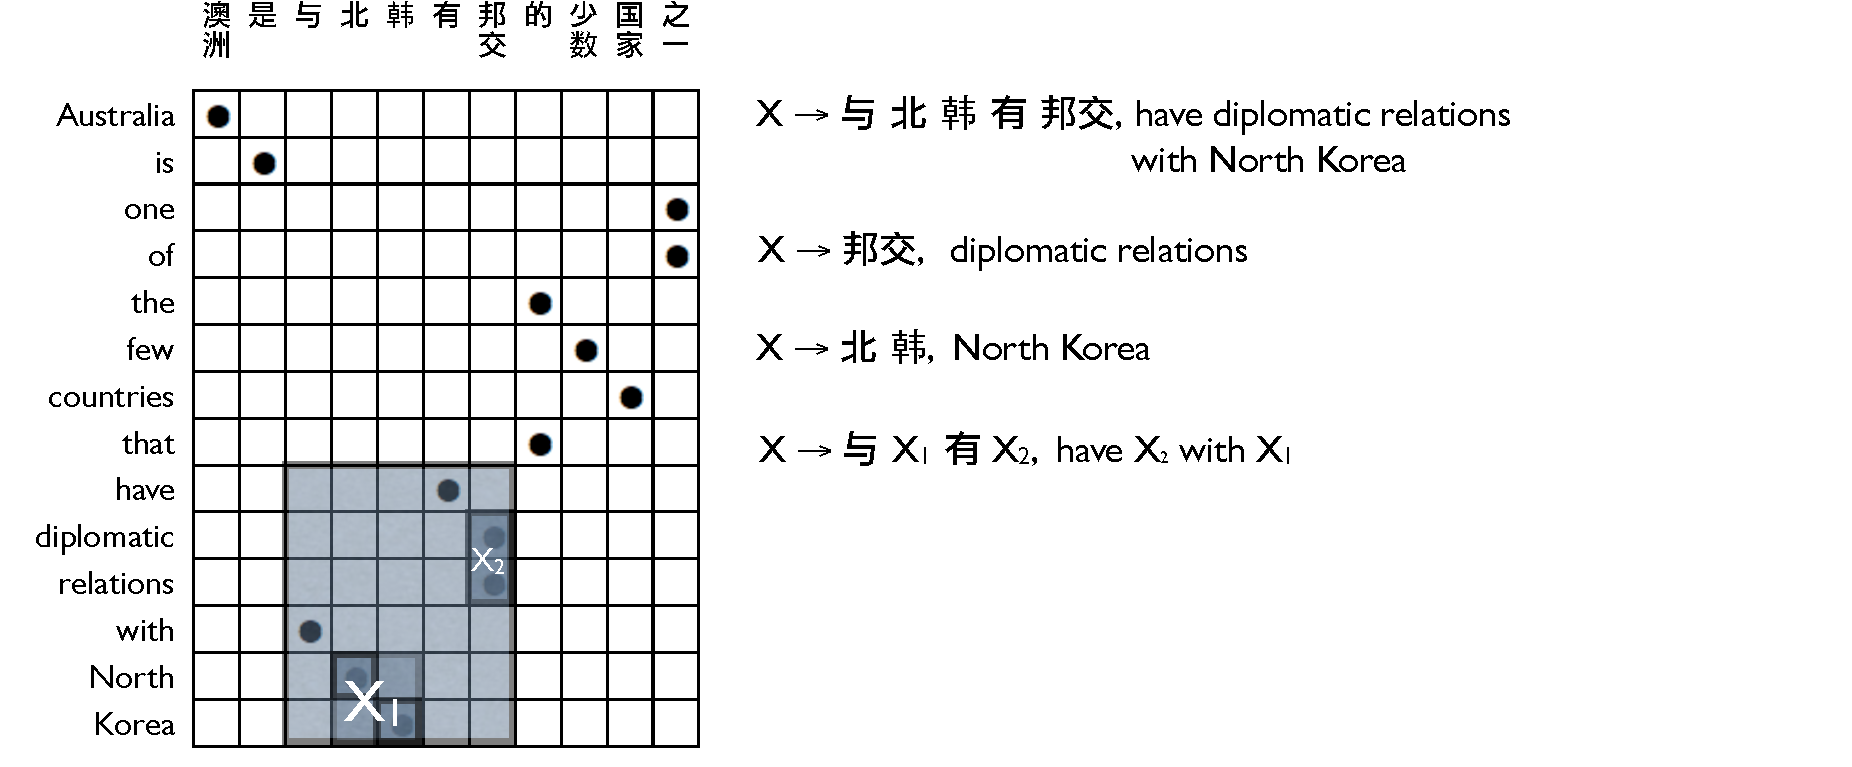
\includegraphics[width=.9\linewidth]{SCFGs/hiero-phrase-extraction.pdf}
\end{center}
\caption{An example of a hierarchal phrase extracted from a word-aligned Chinese-English sentence pair.  Chiang's Hiero system used rules that were written in the form of synchronous grammars, but which are devoid of linguistic information.}\label{hiero-phrase-extraction}
\end{figure}


Rather than using the full power of the SCFG formalism, the Hiero system instead uses a simple grammar with one non-terminal symbol, X, to extend conventional phrase-based models to allow phrases with gaps in them.  The Hiero system is technically a grammar-based approach to translation, but does not incorporate any linguistic information in its grammars.  Its process of decoding is also one of parsing, and it employs the Cocke-Kasami-Younger (CKY) dynamic programming algorithm to find the best derivation using its probabilistic grammar rules.   However, because Hiero-style parses are devoid of linguistic information, they fail to capture facts about Urdu like that it is post-positional or verb final. 

\subsection{Syntax-augmented SCFGs extracted from supervised parses}\label{samt}


\begin{figure}
\begin{center}
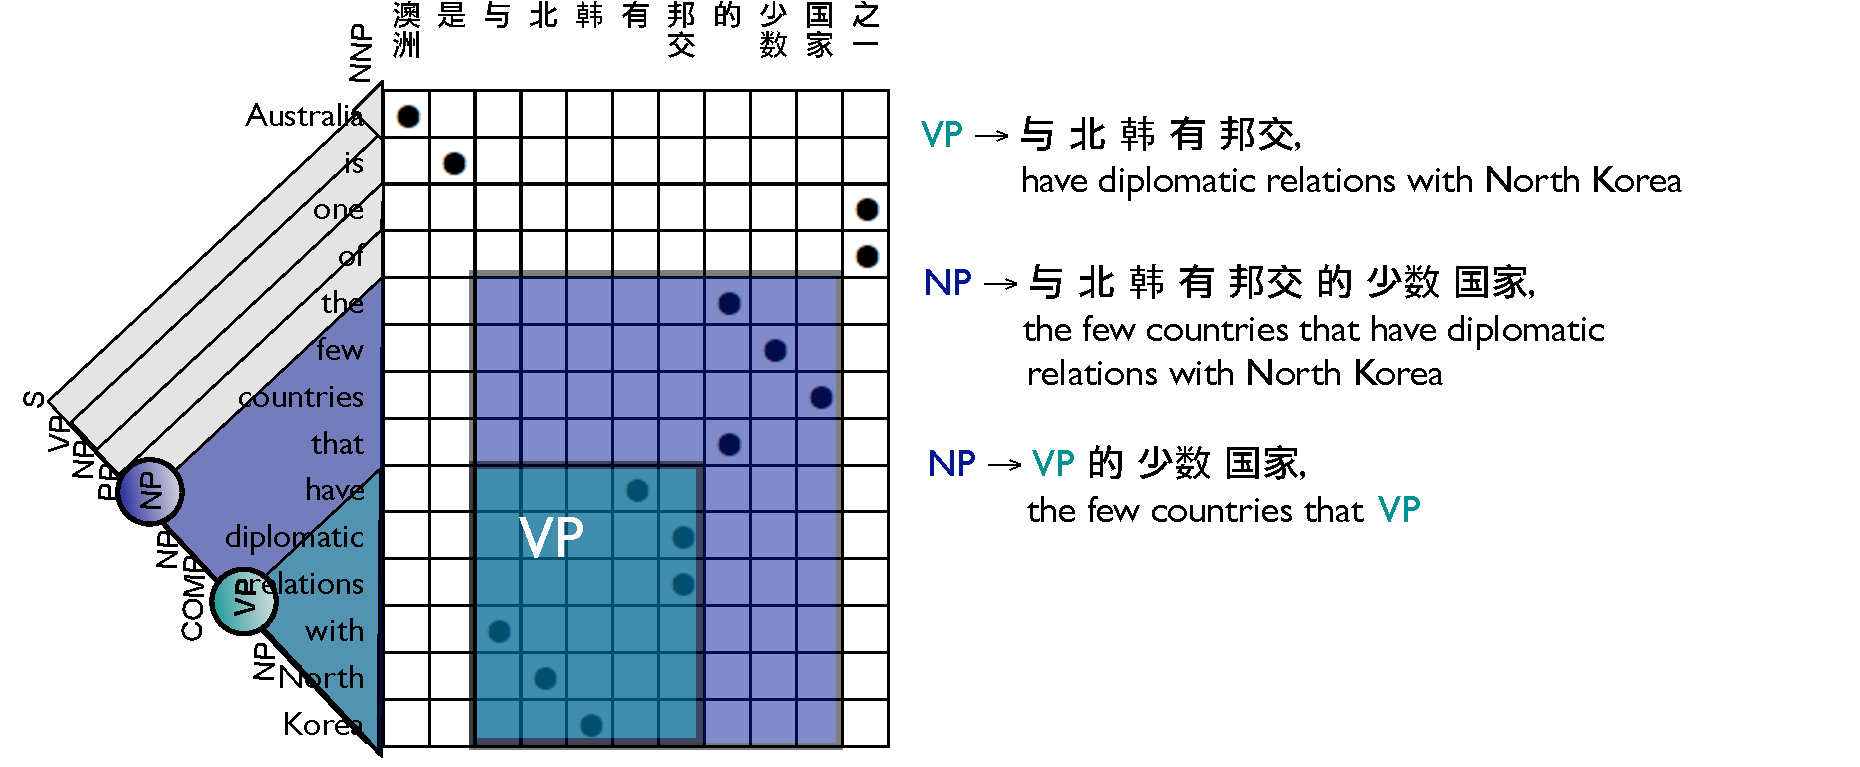
\includegraphics[height=3in]{SCFGs/scfg-phrase-extraction.pdf}
\end{center}
\caption{An example of extracting linguistically-motivated SCFGs by labeling phrase pairs using the labels of the corresponding nodes in a parse tree.  Rules with syntactic non-terminals on the right-hand sides can be formed by replacing  phrase pairs with their non-terminal labels, as shown with the VP on the right hand sides of the second NP rule.}\label{scfg-phrase-extraction}
\end{figure}


SCFGs with a rich set of linguistically motivated non-terminal symbols have been proposed as an alternative to Hiero. A number of approaches have been proposed for extracting linguistically-motivated grammars from a parsed parallel corpus \cite{Galley2004,samt}.   These approaches extract SCFGs from a parallel corpus that has been parsed using a supervised parser that was trained on a treebank.  

Figure \ref{scfg-phrase-extraction} shows how linguistically motivated grammar rules can be extracted from a training sentence pair that has been automatically parsed and word-aligned.    Instead of assigning the generic label ``X'' to all extracted phrase pairs, as the Hiero model does, linguistic labels are extracted from the parse tree.   

In the standard phrase-based and hierarchical phrase-based approaches to machine translation, many of the ``phrases'' that are used are not phrases in the sense of syntactic constituents.  They are simply sequences of words.  For example, in Figure \ref{scfg-phrase-extraction}, the phrases {\it Australia is} and {\it one of} are examples of phrases which have consistent Chinese phrase pairs, but which do not correspond to nodes in the parse tree.  If we were to limit ourselves to extracting only phrase pairs that were licensed by the parse tree and which had consistent word alignments, then we would have reduced coverage compared to Hiero.  Instead, we adopt the methodology described by\citet{samt}, which achieves the same coverage as Hiero by generating complex labels for non-consistuent phrases.  


\begin{figure}
\begin{center}
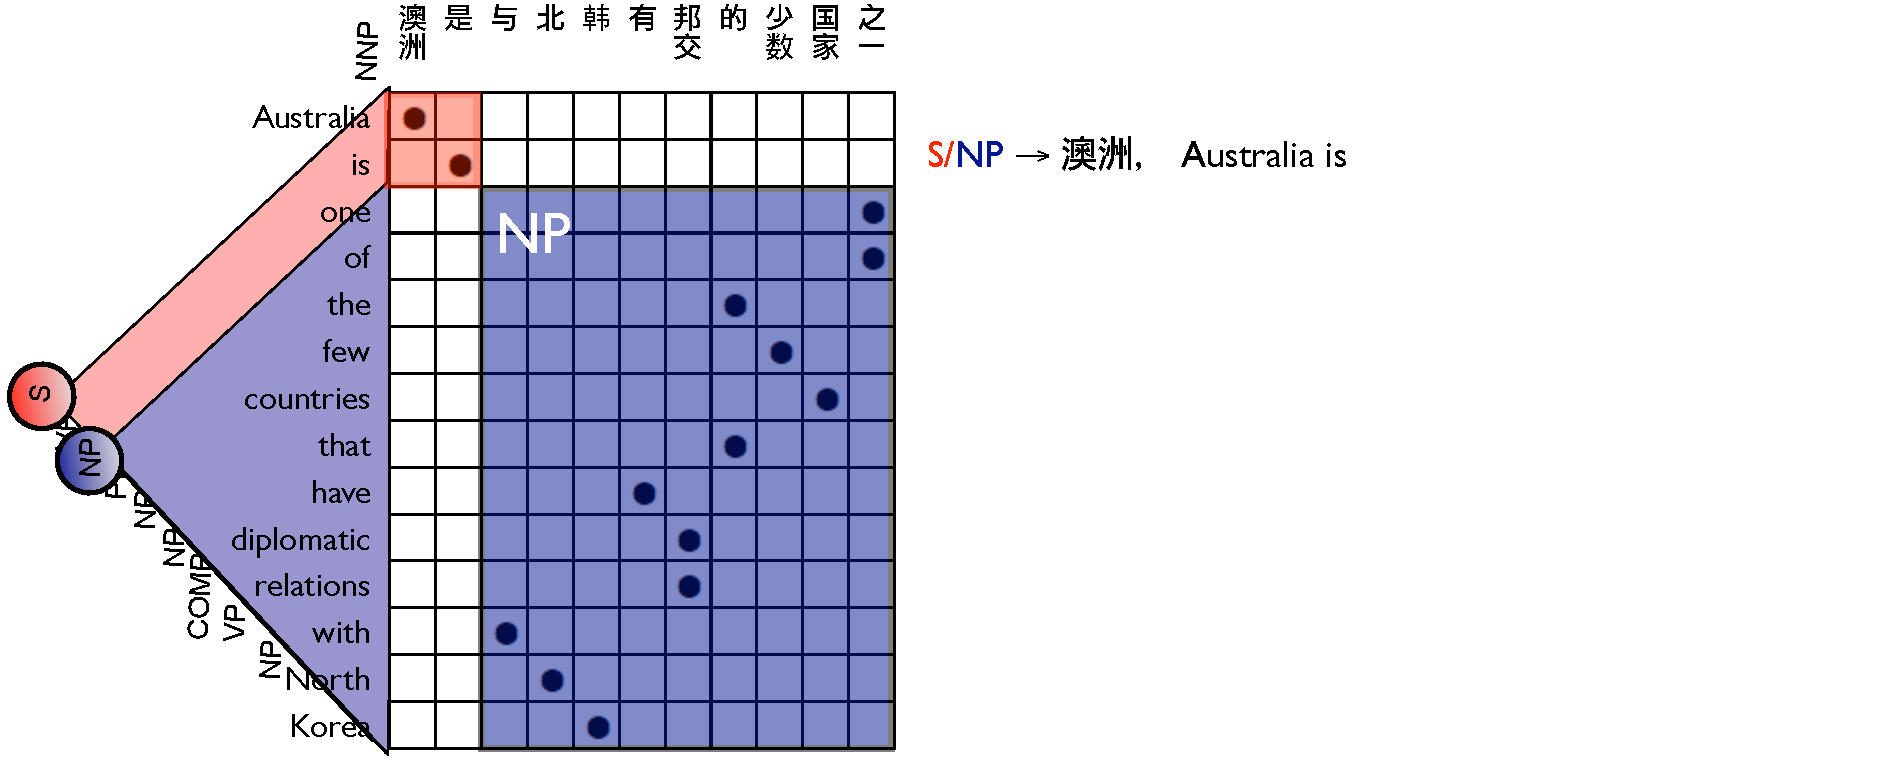
\includegraphics[height=3in]{SCFGs/scfg-ccg-phrase-extraction.pdf}
\end{center}
\caption{An example of a CCG-style label for the non-constituent phrase {\it Australia is}.  The label indicates that the non-constituent phrase would be an S if an NP were found to its right.  This complex label can be treated like any other label during parsing and translation. }\label{scfg-ccg-phrase-extraction}
\end{figure}


\citet{samt} define a framework for extracting SCFGs with linguistically motivated nonterminals from an aligned parallel corpus where one side of the parallel corpus has been parsed. The resulting context-free rules contain a rich set of nonterminal categories. These categories include traditional nonterminal categories taken directly from the monolingual parse trees (e.g. DT, NP, VP), and extended categories formed by gluing together adjacent nonterminals (e.g. NP+V, RB+JJ) and incomplete constituents that denote a category missing a child component to the left (e.g.  NP\textbackslash DT) or to the right (e.g. NP/NN) in the style of Combinatory Categorial Grammars \cite{ccg1982}.   \citet{samt}'s Syntax Augmented Machine Translation (SAMT) grammars may also include hierarchical rules and glue rules \cite{chiang:2007} that are not linguistically motivated; such rules allow partial translations to be combined (with some penalty) without regard to syntactic structure.



\begin{figure}
%\begin{center}
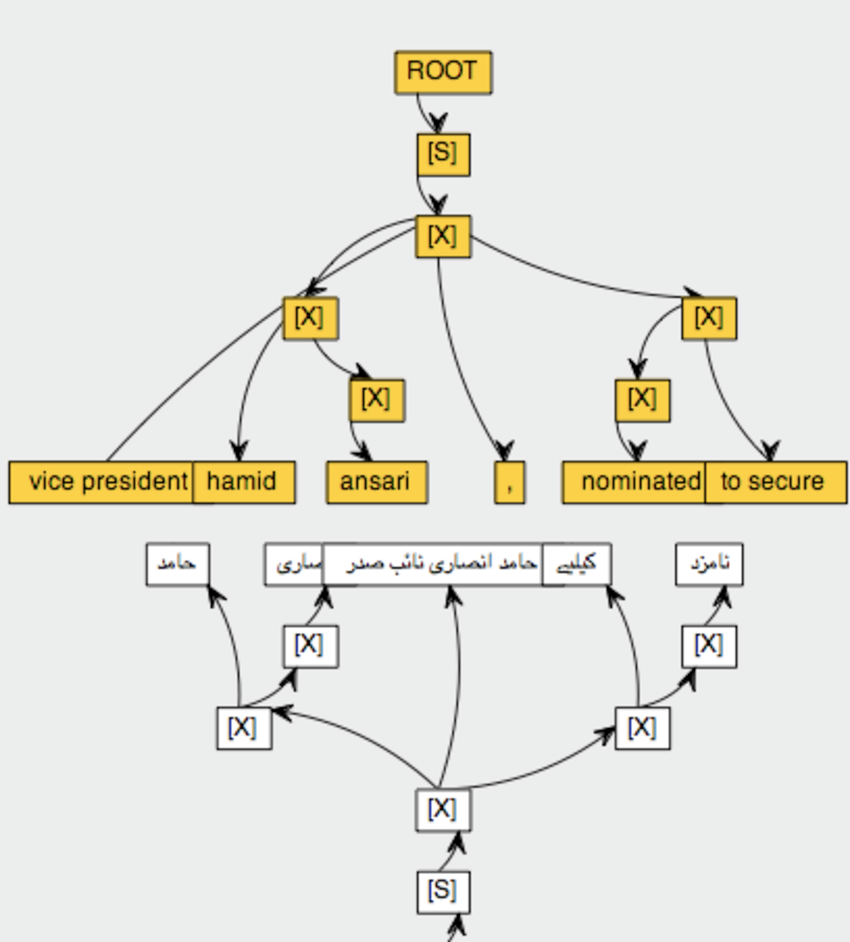
\includegraphics[height=3.75in]{SCFGs/hiero-tree}
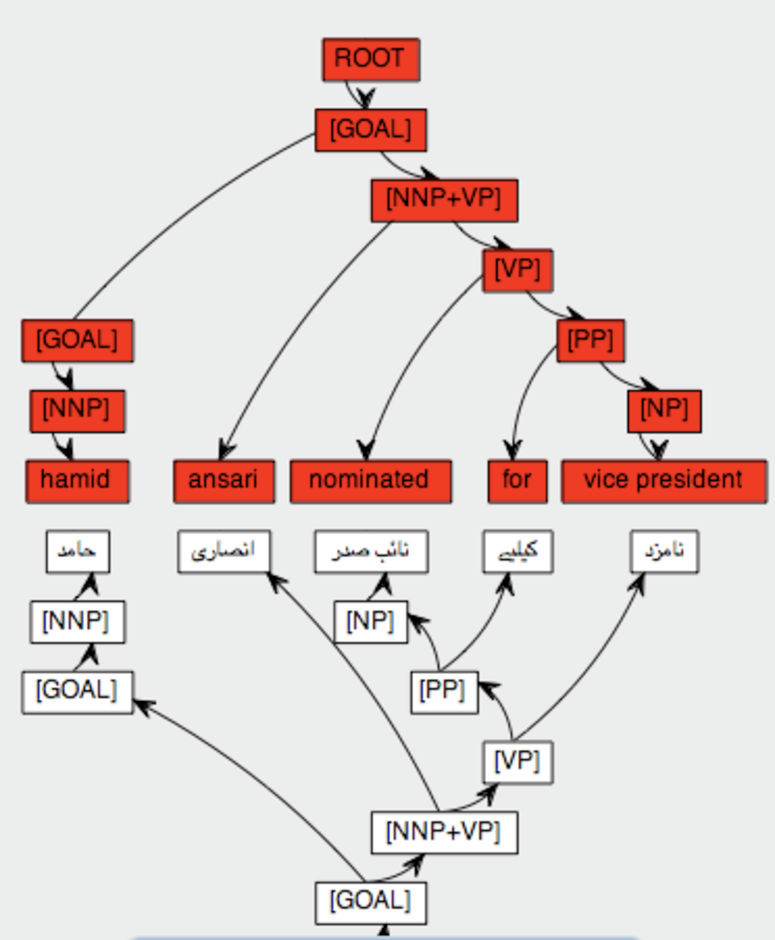
\includegraphics[height=3.75in]{SCFGs/samt-tree}
\caption{Sample derivations for an Urdu sentence translated into English translation using a hierarchical phrase-based SCFG (left) and a linguistically motivated SCFG (right).  For reference, a human translator produced ``Hamid Ansari nominated for the post of vice president" as the translation of the Urdu. }
%\end{center}
\label{example-derivations}
\end{figure}


\subsection{SCFGs with syntactic labels extracted from supervised parses}\label{samt}

Note that one of the major advantages of extracting the linguistic SCFG for an automatically parsed parallel corpus is that only one side of the parallel corpus needs to be parsed.  To extract an Urdu-English SCFG we therefore could use an English parser without the need for an Urdu parser.  During translation the Urdu input text gets parsed with the projected rules, but a stand-alone Urdu parser is never required. 
However, all of the current approaches require that a parser, trained on supervised data, exist for at least one of the languages.  

The methods explored in this summer workshop obviate the need for a supervised parser, and instead automatically induce the grammars from unlabeled texts.  The potential advantages of our approach are:
\begin{enumerate}
\item It can be applied to language pairs for which treebanks do not exist.
\item The set of non-terminal symbols is not tied to a particular treebank formalism, and therefore may be more appropriate for translation.
\end{enumerate} 



\chapter{Experimental Setup}

Our approach is based upon the popular and influential Hiero system \cite{chiang07} which uses a synchronous context free grammar (SCFG) to model translation. 
This translation system uses only a single non-terminal symbol and therefore the system is inherently stateless. 
However, we know that using a richer set of non-terminals can greatly improve translation, as evidenced by the improvments obtained by SAMT system \cite{samt} which augments a Hiero-style SCFG model with syntactic labels.
This is best explained in terms of the generalisation capability: a single category grammar can create all manner of string-pairs, the majority of which are nonsensical and agrammatical, while a model with syntactic categories inherently limits the sets of string pairs to those which are grammatical (largely).
This can be seen from the following example rules, showing how rules can be combined to arrive at ungrammatical string pairs.
\begin{align*}
X &\rightarrow \langle \mbox{does not}~X, \mbox{ne}~X~\mbox{pas} \rangle \\
X &\rightarrow \langle \mbox{cat}, \mbox{chat} \rangle \\
X &\Rightarrow \langle \mbox{does not cat}, \mbox{ne cat pas} \rangle
\end{align*}

As such, the single-category model licenses all manner of word-salad output, thus relying on the language model to salvage a coherent sentence from these options.
In contrast, the set of translation options for the grammar with syntactic labels is much smaller and more coherent, and thus the language model has less heavy lifting to do.
This setting plays well to the strengths of a n-gram language model which can accurately model local coherence but is unable to model global sentence-level effects (which are modelled by the syntactic translation model). 
%In addition, a treebank parser and an n-gram language model have different strengths -- the parser can ensure more global grammatical coherence but over-generalises at the lexical level, while the n-gram model does the opposite.

The central aim of the project was to induce automatically a rich translation grammar to realise some of the performance gains resulting from the use of linguistic grammars, but without using linguistic resources such as treebank parsers.
This allows our approach to be more easily ported to work for translating a variety of languages, rather than being constrained to just translating into languages with good syntactic resources (typically English).

\section{Distributional Hypothesis}

Underlying most models of grammar induction is the distributional hypothesis. This theory states that
``words that occur in the same contexts tend to have similar meaning'' \cite{harris:54}. Although phrased in terms of semantics, the distributional hypothesis applies equally to syntax, that is, words that can be substituted for one another most often share the same syntactic category (in general, semantics implies syntax). This is evidenced by the wide-spread use of the substitution test in theories of syntax to determine the constituency and syntactic category of a word or phrase.

The majority of work on monolingual grammar induction has used some notion of context to inform the induced categories. This is best seen in the work of Alex Clark who uses the context surrounding a phrase to determine its category, and in Dan Klein's work, which uses context to determine constituency. In this project we follow the lead of these earlier works on monolingual grammar induction by using context to inform our clustering of words and phrases, such that words that appear in similar contexts are assigned to the same cluster. We expect that this clustering should bear a strong resemblance to the underlying syntax and, to some extent, the semantics of the language, and therefore improve translation accuracy.

Our bilingual translation setting differs from the earlier monolingual settings in which most grammar induction research has been performed. We seek to label a broad range of n-grams (so-called phrases) as supplied from the phrase extraction process. These n-grams will be both constituents and non-constituents. The use of non-constituent translation units has been shown consistently to outperform systems which use only constituents in terms of translation quality. For this reason how grammar induction system must be able to infer useful syntactic categories for these non-constituent n-grams.

\section{Clustering Configuration}

Notion of context.
Mono/source/target/bi, words/classes/POS.
Give example.
Notation.

\begin{table}
\begin{tabular}{cp{.7\textwidth}}
\toprule
  symbol & meaning \\
\midrule
  $\mathbf{p} = (p_1, \ldots, p_n)$ & a phrase (n-gram) of word tokens \\
  $\mathbf{c} = (\ldots, c_{-2}, c_{-1}, c_1 c_2, \ldots)$ & a context of immediate words surrounding a phrase, with the index signifying the distance to the left (negative indices) or right (positive indices) of the phrase \\
  $e = (p, c)$  & a edge denoting a phrase, $p$, occuring in context $c$ \\
  $z$ & label assigned to an edge, denoting the cluster or non-terminal assigned to the phrase in context \\
  $K$ & number of clusters, $z \in \{1,2, \ldots, K\}$ \\
  $P$ & set of unique phrases \\
  $C$ & set of unique contexts \\
  $C_p$ & set of contexts in which $p$ has occurred \\
  $P_c$ & set of phrases occuring in context $c$ \\
\bottomrule
\end{tabular}
\caption{Notation used throughout this paper.}
\end{table}

\section{Pipeline}

Brief overview of the pipeline. 

\subsubsection{Phrase Extraction}

\section{Evaluation}

We evaluate the output of the pipeline in the standard way. But in order to short-cut the lengthy process we also evaluate the quality of the clustering against linguistic labellings.

\subsubsection{BLEU}

\subsubsection{Conditional Entropy}

\[ H(S|Z) = \sum_{s,z} p(s,z) \log \frac{p(z)}{p(s,z)} \]

%%% Local Variables: 
%%% mode: latex
%%% TeX-master: "report"
%%% End: 


\newcommand{\p}{\textbf{p}}

\chapter{Nonparametric Models}

In this chapter we describe several closely related Bayesian nonparametric models for inducing categories in a synchronous context-free grammar.  Our nonparametric models are variations on Latent Dirichlet Allocation (LDA) model of \cite{blei:2003}.  Rather than modeling sentences (or sentence pairs), we assume that rule extraction heuristics determine the set of valid constituents and grammar rules, and so our task is only to determine the category labels.  As discussed in the previous chapter, we make the critical assumption that each phrase (or pair), $\p$, can be clustered on the basis of the contexts it occurs in.  We therefore define a generative model of a corpus that consists of collections of contexts (one context collection for each phrase pair type).

\section{Model}

The high-level structure of our model is as follows: each observed phrase (pair), $\p$, consists of a finite mixture of categories, $\theta_{\p}$.  The list of contexts $C_{\p}$ is generated as follows.  A category type $z_i$ is drawn from $\theta_{\p}$, and this generates the observed context, $\textbf{c}_i$, according to a category-specific distribution over contexts types, $\phi_{z_i}$.  Since we do not know the values of $\theta_{\p}$ and $\phi_z$, we place priors on the distributions, to reflect our prior beliefs about the shape these distributions should have and infer their values from the data we can observe.  Specifically, our {\emph a priori} expectation is that both parameters will be relatively peaked, since each phrase, $\p$, should relatively unambiguous belong to particular category, and each category to generate a relatively small number of context strings, $\textbf{c}$.

To encode these prior beliefs, we make use of Pitman-Yor processes \citep{pitman:1997}, which can capture these intuitions and which have already been demonstrated to be particularly effective models for language \citep{teh:2006,goldwater:2006}.

Our models assume a fixed number of categories, $K$. The category type, $z \in \{ 1 , 2 , \ldots , K \}$, is generated from a PYP with a uniform base distribution:
\begin{align*}
z &| \p & \sim \theta_{\p} \\
\theta_p &| a_{\p},b_{\p},K & \sim \textrm{PYP}(a_{\p},b_{\p},\textrm{Uniform}(K))
\end{align*}
\noindent Alternatively, we used hierarchical PYP process which shares statistics about the use of categories across phrases:
\begin{align*}
z &| \p & \sim \theta_{\p} \\
\theta_{\p} &| a_{\p},b_{\p} & \sim \textrm{PYP}(a_{\p},b_{\p},\theta_0) \\
\theta_0 &| a_0,b_0,K & \sim \textrm{PYP}(a_0,b_0,\textrm{Uniform}(K))
\end{align*}

\noindent Each category $z$ token then generates the context $\textbf{c}_i$. We again model this using a PYP, which will tend to cluster commonly used contexts across phrases into a single category. Additionally, by using hierarchical PYPs, we can smooth highly specific contexts by backing off to less specific contexts (e.g., composed of fewer words or word classes).

The most basic version of our model uses a uniform prior base distribution over contexts:

\begin{align*}
\textbf{c} |& z & \sim \phi_z \\
\phi_z |& a_z,b_z & \sim \textrm{PYP}(a_z,b_z,\textrm{Uniform}(|V|^2))
\end{align*}

\noindent TODO. For contexts with more than a single word on either side, we typically backed off from a 

\begin{align*}
\textbf{c} |& z & \sim \phi_z \\
\phi_z |& a_z,b_z, \phi_0 & \sim \textrm{PYP}(a_z,b_z,\phi_0(\cdot|z) \times \textrm{Uniform}(|V|^2)) \\
\phi_0 |& a_0,b_0 & \sim \textrm{PYP}(a_z,b_z,\phi_0(\cdot|z))
\end{align*}

\noindent Figure~\ref{fig:np_plate} shows a plate diagram for the model.

\begin{figure}
\begin{center}
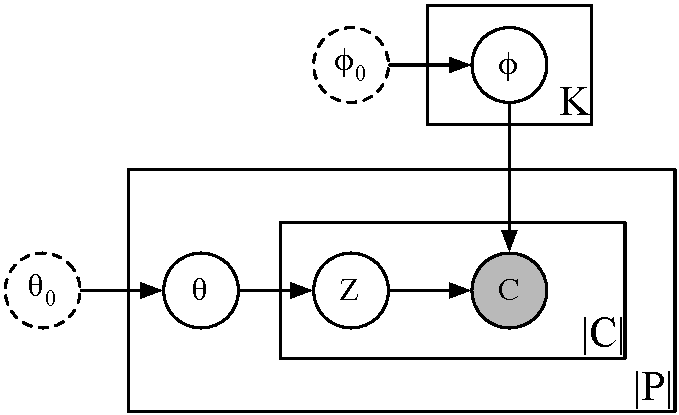
\includegraphics[scale=0.75]{pyp_clustering/np_plate.pdf}
\vspace{-0.3cm}
\end{center}
\caption{Plate diagram for the nonparametric clustering model (hyperparameters omitted).  Dashed circles indicate variables that may not be present in every model.}
\label{fig:np_plate}
\end{figure}

\subsection{Inference}

Inference in this model was performed using Gibbs sampling \citep{geman:1984}, with the continuous parameters ($\theta_{\p}$, $\phi_z$, etc.) integrated out.  For the experiments reported below, we sampled for 1000 iterations, initializing by assigning every context in a phrase entirely to a random category.  New values for the PYP hyperparameters were resampled using slice sampling every 10 samples \citep{neal:2000,johnson:2009}. The final sample was used to estimate $p(z|\textbf{c},\p)$, and each phrase occurrence was labelled with the $z$ that maximized this probability (TODO check this).

\section{Experiments}

\subsection{Number of categories}

\subsection{Context types}



\newcommand{\gloss}[1]{\glossa{(#1)}}%\begin{small}\textit{(#1)}\end{small}}
\newcommand{\glossa}[1]{\begin{small}\textit{#1}\end{small}}
\newcommand{\pemph}[1]{\textbf{#1}}
\newcommand{\mmsz}{0.4\textwidth}
\newcommand{\mmultirow}[2]{\multirow{#1}{\mmsz}{#2}}

\chapter{Inducing Morphological Structure}

In this chapter, we evaluate the application of our grammar induction method to the problem of translating at the morphology level.

\section{Introduction}
Mainstream SMT research mostly ignores morphological variation, treating translation as a mapping of words and phrases from a source to a target language without taking cognisance of word-internal structure.
This approach has worked reasonably well for various languages, but is ill-suited for language pairs with substantial morphological divergence, e.g. Turkish and English.

Morphological variation is a source of sparseness in the training that can make it hard or impossible to produce correct translations of word forms not observed during training, or observed only rarely.
The sparseness problem can of course be mitigated by using ever larger sets of training data, but for anything short of an infinite parallel corpus, a language with relatively expressive morphology should succeed in producing word forms that simply never appear in the corpus.
This is especially true for languages with complex morphology like Turkish, Finnish and Hungarian, where there is a proliferation of word forms.

Ideally, we would like to leverage the words observed in the training data to generate differently inflected forms of them.
For example, the correct conjugation of the French verb for ``(we)~hear'' could be generated as illustrated below, where boldface and underlining mark the origins of the relevant word segments:

\begin{figure}[h]
%\label{fig:inflection}
\centering
	\begin{tabular}{rlcll}
	\multicolumn{2}{c}{\textbf{\textit{Observed}}} 	&  & \multicolumn{2}{c}{\textbf{\textit{Generated (not observed)}}} \\[5pt]
	\gloss{I hear} & j'\textbf{entend}s 
		&  \multirow{2}{*}{$\Longrightarrow$} 
		& \multirow{2}{*}{nous \textbf{entend}\underline{ons}} 
		& \multirow{2}{*}{\gloss{we hear}} \\ 
	\gloss{we reply} & nous r\'{e}pond\underline{ons} 	&  &  	& 
	\end{tabular} 
%\caption{Learning from morphemes: Boldface and underlining trace the elements used to form the unobserved word. English translations are given in parentheses.}
\end{figure}

In general, our aim here is to identify morphemes in the observed words and combine them correctly to generate novel word forms.
To achieve this, we require rules for how morphemes may combine.
Such rules could be hand-crafted for a particular language, but in keeping with the spirit of statistical MT, we strive toward language independent solutions and would rather induce rules from data.
A SCFG could be suitable for expressing such rules, so how about we use the grammar induction methods discussed earlier to obtain one that is capable of translating morphemes.
In particular, the plan is to have a single grammar deal with morpheme combination (i.e. word formation) as well as sentence formation.
This is the central idea for this chapter and is developed further in the next section.

\paragraph{Work this in somewhere}
Morphology has received attention in SMT research before, with reasonable success both
 when the source language has richer morphology than the target language \citep{Yang2006,Dyer2008}, 
 and vice versa \citep{someone,Yeniterzi2010} .
To our knowledge, Dyer08 is the only other case where morphology has been targeted in the context of a translation system that uses SCFG for transduction.

In the monolingual setting, morphology has been modelled with 
rule-based finite-state automata \citep{someone}, 
unsupervised methods \citep{Creutz2006,Goldsmith2001},
 .. lookup those leads from workshop feedback]. Highlight what is novel/unique about our approach.

\section{Motivation for a Labelled Grammar}
We use the Hiero-grammar with its single non-terminal category, X, as a starting point and imagine that we induce it from a corpus that has been segmented into morphemes.
For the moment, we ignore the fact that this grammar is synchronous.
Observe that a context-free grammar can be employed to generate words from morphemes, as shown by the grammar fragment and derivation of ``enabled'' in Figure \ref{fig:m_motivation_x}.

Yet the same grammar fragment also licenses the production of nonsense, such as ``enablely''.
This is because this grammar does not enforce proper restrictions on morpheme attachment, allowing a string like ``+ly address'' to attach to ``enable+'' as a `suffix'.

We use the `+' character to mark morpheme boundaries.
Apart from being a a display device, it also creates a distinction in the vocabulary if some token exists 
both as a morpheme and a word in its own right.
But it is insufficient for enforcing proper attachment, even if the grammar were aware of the marker's meaning.

\subfigcapskip=15pt
\begin{figure}[h]
  \centering
  \subfigure[Non-sensical words can be produced when using a single non-terminal category.]{\label{fig:m_motivation_x}
  \begin{tabular}{rcl}
    \begin{minipage}{0.3\textwidth}
      \begin{tabular}{lcl}
        X & $\rightarrow$ & en+ +able+ X \\
        X & $\rightarrow$ & +d \\
        \textit{X} & $\rightarrow$ & \textit{+ly address} \\
      \end{tabular}
    \end{minipage}
    &
    \begin{minipage}{0.3\textwidth}
      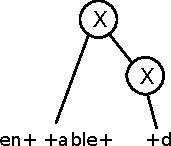
\includegraphics[scale=1]{morphology/treelet_good}
    \end{minipage}
    &
    \begin{minipage}{0.3\textwidth}
      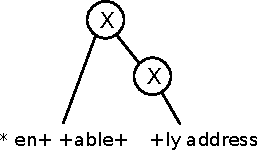
\includegraphics[scale=1]{morphology/treelet_bad} 
    \end{minipage}
    \\
  \end{tabular}
  }

  \subfigure[Constraining the grammar with labelled rules can avoid the problem.]{\label{fig:m_motivation_labelled}
  \begin{tabular}{rl}
    \begin{minipage}{0.4\textwidth}
      \begin{tabular}{lcl}
        X & $\rightarrow$ & en+ +able+ \textbf{X3} \\
        \textbf{X3} & $\rightarrow$ & +d \\
        X & $\rightarrow$ & +ly address \\
      \end{tabular}
    \end{minipage}
    &
    \begin{minipage}{0.3\textwidth}
      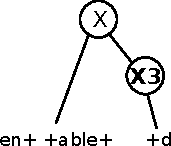
\includegraphics[scale=1]{morphology/treelet_good_label}
    \end{minipage}
    \\[10pt]
  \end{tabular}
  }
  \caption{Grammar fragments and possible derivations they allow when using a single category (top) vs. multiple categories (bottom).}
  \label{fig:m_motivation}
\end{figure}
\subfigcapskip=10pt

To solve the problem, we wish to constrain the grammar by using more refined non-terminal categories.
Specifically, we do not want the word-forming and sentence-forming rules of the grammar to mix.
Thus we propose to use a set of labelled categories for word-formation, disjoint from X.
With the modified grammar fragment shown in Figure \ref{fig:m_motivation_labelled}, the non-sensical word can no longer be produced.

These examples only serve to illustrate word formation in the monolingual case.
Of course, we are actually operating in a bilingual situation and using synchronous CFGs.
Thus, another merit of this approach is that it can capture morpheme reordering in a natural way. (Example).

\section{Morpheme Clustering and Labelling}
By no mere coincidence, we have a suitable source of the aforementioned kind of labelled grammar rules in the form of the clustering method described in chapter \ref{chap:np_clustering}.
We will use it to cluster morphemes depending on their context within words.
To this end we use the normal phrase extraction heuristics on a corpus that has been segmented into morphemes.
Thus in the terminology introduced earlier in this report, a phrase $\mathbf{p}$ and its context $\mathbf{c}$ are both sequences of morphemes, as illustrated below.
Importantly, we only perform the clustering on phrases not containing word boundaries, since we are specifically after rules of word formation.

\begin{figure}[h]
\begin{tabular}{ll}
\textit{Original sentence:}\footnote{Gloss: \gloss{changes have no place to be}} & les modifications n' ont pas lieu d' \^{e}tre \\[3pt]
\textit{Segmented sentence:} &
 $\underbrace{\textrm{les}}_{c_{-1}} \;
	\underbrace{\textrm{modifi+}}_{\mathbf{p}} \;
	\underbrace{\textrm{+cation+}}_{c_{+1}}$ \; +s n' ont pas lieu d' \^{e}tre \\[8pt]
 \multicolumn{1}{r}{$\Rightarrow$} 
 	 & $\mathbf{p}= (\textrm{modifi+}),$ \\
 	 & $\mathbf{c} = (c_{-1},c_{+1}) = (\textrm{les, +cation+})$
\end{tabular}
\end{figure}

The underlying assumption made by applying this clustering method is that a morpheme's context is indicative of its substitutability.
The previous example is an instance of noun derivation from a verb stem.
In order to form other nouns by this mechanism, different verb stems need to be substituted in place of ``modifi+''.
This can be achieved if the appropriate morphemes occurring in this context are clustered together under the same label, say, $z=15$:

\begin{center}
\begin{tabular}{ccl|ccl}
les & modifi+  & +cation+ & les & justifi+ & +cation+ \\
 & X15 &  & & X15 & \\
\end{tabular}
\end{center}

Morphemes in the training corpus are labelled in this way, based on the categories induced by clustering.
This still leaves many spans in the corpus unlabelled, in particular those that contain word boundaries.
During grammar extraction, these spans give rise to the sentence-forming X-rules, whilst the labelled spans yield the word-forming labelled rules, as detailled previously.

\section{Experimental Setup}
The ideas expressed above need to be verified empirically.
The most direct approach was to do this somewhat isolated from the other workshop experiments.
In other words, we used a Hiero-grammar as the starting point and used the clustering to learn morpheme combination rules only.
We did not also apply it to words and phrases, although that was starting to show the improved BLEU scores reported elsewhere in this document.

We chose Dutch and French as a test language pair, since 1) they both have a fair amount of interesting inflection and 2) it was the most suitable language pair from amongst those for which suitable training data was prepared before the workshop.

\subsection{System Description}

\paragraph{Data}
We filtered the training corpus down to the first 100k sentence pairs that contain at most 40 words per sentence.
The word limit was imposed because the actual number of tokens in a sentence will be higher once it is segmented into morphemes.
This was a time-saving shortcut on various fronts: It restricts the size of the extracted grammars and therefore the decoding time too, and, more importantly, allowed us to obtain the new word alignments and language model in a reasonable amount of time.
It also makes the alignment task slightly less error-prone, although this remains problematic and is discussed in section \ref{sec:m_analysis}.

\paragraph{Segmentation}
For word segmentation, we used the unsupervised Morfessor Categories-MAP algorithm \citep{Creutz2007}, which is based on a HMM.
It induces a word segmentation model from a monolingual corpus, where a word consists of one or more stem morphemes with zero or more prefixes and/or suffixes, each marked as such.
Since we weren't interested in how well Morfessor can segment words it did not observe during its training stage, we trained a segmentation model on the complete training, development and test data that will be used by the translation system.
We did not make use of the induced morpheme categories (prefix, stem, suffix), but simply applied the segmentation models to split the training, development and test data into generic morphemes.

The granularity of segmentation is controlled by specifying a perplexity threshold ($PPL$ in the Morfessor configuration file).
After some informal tests on a small data set, we chose $PPL_{\textrm{Dutch}}=300$ and $PPL_{\textrm{French}}=150$.
Table \ref{tbl:segmentation} summarises the effect this had on the (MT) training data.

\begin{table}[h]
  \centering
  \begin{tabular}{|l|l|r|r|}
    \multicolumn{2}{c}{} & \multicolumn{1}{c}{Dutch} & \multicolumn{1}{c}{French} \\ \hline
    \multirow{2}{*}{Types}  & words     & 43611 & 35225 \\ \cline{2-4}
                            & morphemes & 26409 & 21962 \\ \hline
    \multirow{2}{*}{Tokens} & words     & 2035254 & 2180898 \\ \cline{2-4} 
                            & morphemes & 2647203 & 2874574 \\ \hline
  \end{tabular}
  \caption{x}\label{tbl:segmentation}
\end{table}

\paragraph{Grammar Induction Parameters}
We obtained two grammars for testing, one by clustering the source side and the other on the target side.
Following from other workshop results, we chose $K=25$ categories, although our setting here is rather different.
Morpheme sequences of at most $|\mathbf{p}|=10$ were obtained from the aligned, segmented corpus using the standard phrase extraction method and context was chosen as one token either side of such a sequence, i.e. $\mathbf{c}=(c_{-1},c_{+1}$.
The non-parametric model with hierarchical Pitman-Yor Process priors was run for a 1000 samples in each case and the last sample used to label morpheme sequences.
The resulting grammars each have a total of 26 non-terminal categories: the default X category plus the 25 labelled categories.

\paragraph{Translation System}
Word alignments were trained on the segmented parallel corpus using the Berkeley Aligner \citep{Liang2006} with default settings.

A French language model over morpheme n-grams was also required.
3-gram language models were used throughout the workshop.
But due to word segmentation, the number of tokens in the French training corpus, and therefore the average number of tokens per sentence, increased by 32\% (Table \ref{tbl:segmentation}).
We therefore opted for a 4-gram language model, since that yields, on average, three full words of context, thus corresponding to a 3-gram model on unsegmented data.

\section{Results}

\subsection{Intrinsic Evaluation}
In order to gain some insight into the quality of the morpheme clustering, we scrutinised cluster contents for obvious patterns.
This was done only for the case where the clustering was done on Dutch (source language), since expertise was available there but not in French.
Some of the observations are summarised in Table~\ref{tbl:m_cats}. 

\begin{table}[hbt]
  \centering
    \begin{tabular}{c|p{\mmsz}|l}
    \textbf{$z$} & \textbf{Description} & \textbf{Examples} \\
                 &                      & format: $c_{-1}$ \p\ $c_{+1}$  \gloss{translation} \\ \hline
    0 & \parbox{0.4\textwidth}
        {75\% concerns the infix +s+, both as \p\ and as $c_{+1}$} &
        \begin{minipage}{0.4\textwidth}
          \begin{tabular}{ll} 
            de \pemph{europe+} +s+ & \gloss{the european+} \\
            europe+ \pemph{+s+} +e & \gloss{european}
          \end{tabular}
        \end{minipage} \\ \hline

    1 & \parbox{0.4\textwidth}
        {$>$85\% prefix morphemes as \p, mostly noun stems with plural forming $c_{+1}$.} &
        \begin{minipage}{0.4\textwidth}
          \begin{tabular}{ll} 
            ... \pemph{resolutie+} +s & \gloss{resolutions} \\
            ... \pemph{kilometer+} +s & \gloss{kilometres} \\
          \end{tabular}
        \end{minipage} \\ \hline

    4 & \parbox{0.4\textwidth}
        {$>$99\% verb stems as \p} &
        \begin{minipage}{0.4\textwidth}
          \begin{tabular}{ll} 
            ge+ \pemph{+maakt} ... & \gloss{made} \\
            ver+ \pemph{+werpt} ...& \gloss{reject(s) [verb]} \\
            samen+ \pemph{+brengt}...& \gloss{bring together} \\
          \end{tabular}
        \end{minipage} \\ \hline

    5 & \parbox{0.4\textwidth}
        {25\% \p-instances are the prefix ``ver+''. \\ 
         25\% \p-instances are the domain-specific suffix ``+missie''. \\ 
         14\% $c_{+1}$-instances are the adjective-deriving suffix ``+isch''.} &
        \begin{minipage}{0.4\textwidth}
          \begin{tabular}{ll} 
            ... \pemph{ver+} +slag & \gloss{report} \\
            ... \pemph{ver+} +beter & \gloss{improve} \\
            com+ \pemph{+missie} ... & \gloss{commission} \\
            ?? isch \\
          \end{tabular}
        \end{minipage} \\ \hline

    6 & \parbox{0.4\textwidth}
        {$>$99\% adjective stems, followed by a marker for definiteness.} &
        \begin{minipage}{0.4\textwidth}
          \begin{tabular}{ll} 
            ...\pemph{interessant+} +e & \gloss{interesting} \\
            ...\pemph{etisch+} +e & \gloss{ethical} \\
          \end{tabular}
        \end{minipage} \\ \hline

    7 & \parbox{0.4\textwidth}
        {$\pm$13\% are stems followed by ``+elijk'', often forming adverbs(?). \\
         $\pm$17\% are noun-deriving suffixes ``+heid''/``+heden''.} &
        \begin{minipage}{0.4\textwidth}
          \begin{tabular}{ll} 
            ...\pemph{aanvank+}  +elijk & \gloss{initially} \\
            ... \pemph{begrijp+}  +elijk & \gloss{understandably} \\
            vrij+  \pemph{+heden}  ... & \gloss{liberties} \\
            bevoegd+ \pemph{+heid}  ... & \gloss{authorisation} \\
          \end{tabular}
        \end{minipage} \\ \hline

    10 & \parbox{0.4\textwidth}
        {72\% full words, mostly (compound) nouns or things acting as such. Where $c_{-1}$ is an article, nouns are almost exclusively neuter singular.} &
        \begin{minipage}{0.4\textwidth}
          \begin{tabular}{ll}
            het \pemph{uit+breken}  van & \gloss{the outbreak of} \\
            ... \pemph{drie+jaren+plan}  ... & \gloss{three-year plan} \\
          \end{tabular}
        \end{minipage} \\ \hline

    16 & \parbox{0.4\textwidth}
        {$>$92\% full words, similar to but much larger than Cat. 10. Where $c_{-1}$ is an article, nouns are almost exclusively plural or male/female singular.} &
        \begin{minipage}{0.4\textwidth}
          \begin{tabular}{ll}
            de \pemph{wet+geving}  van & \gloss{the legislation of} \\
            deze  \pemph{wij+zig+ing}  ... & \gloss{this modification} \\
          \end{tabular}
        \end{minipage} \\ \hline
  \end{tabular}


  \caption{A selection of observations about the outcome of clustering morpheme sequences in the source language (Dutch). Cluster sizes ranged from X to Y.}
  \label{tbl:m_cats}
\end{table}

The quality of unsupervised clustering is generally tricky to judge.
In our case, it involves determining whether the clusters encode useful ``rules'' for morpheme combination.
There are strong indications that certain worthwhile patterns are learned and that the clustering is therefore partially successful.
To highlight some, note in Table~\ref{tbl:m_cats} that categories~4 and 6 involve a clear separation between two high-level parts of speech, and that a fine-grained distinction about Dutch nouns was learned in categories~10 and 16.

On the other hand, there are ample examples of conflation. Sometimes there is little or no useful linguistic pattern that can be discerned.
As an example, the conflation shown for category~0 implies that both ``europe+'' and ``+s'' will receive the same label, which would give rise to the kind of unrestricted substitutability that we wanted to avoid, as explained in Figure~\ref{fig:m_motivation}.

\subsection{Extrinsic Evaluation}
Ultimately, performance in translation is what matters.
The main question is what impact clustering has when applied to segmented training data.
The baseline system is therefore trained on the same segmented data but without the clustering, i.e. using the Hiero grammar.
For further comparison, we also include the score Hiero achieves on the same training data in its original, unsegmented form.

Table \ref{tbl:m_bleu} gives the final BLEU scores.

\begin{table}[htb]
  \centering
  \begin{tabular}{|l|c|c|c|} \hline
     & \textbf{OOV} & \textbf{BLEU}(m) & \textbf{BLEU} \\ \hline 
    Hiero (\textbf{baseline}) & x & 20.92  & \textbf{15.57} \\ \hline
    Source clustered & x & 20.63 & \textbf{15.37} \\ \hline
    Target clustered & x & 20.66 & \textbf{15.42} \\ \hline
    \multicolumn{3}{c}{ } \\ \hline
    Hiero, original data & x & 20.55 & \textbf{15.67} \\ \hline
  \end{tabular}
  \caption{Results, averaged over 3 MERT runs. BLEU(m) is calculated on the segmented output (i.e. the actual output in the first three cases), whereas last column contains the final scores after recombining the output morphemes into words.}
  \label{tbl:m_bleu}
\end{table}

\subsection{Analysis} \label{sec:m_analysis}
The fact that our approach degraded translation quality as measured by BLEU can be attributed to various factors.

The primary reason is that the word segmentation introduces (additional) errors into the bilingual token alignments.
The alignments are crucial, since they determine the phrases (morpheme sequences) that are extracted and input to the clustering and grammar extraction algorithms.
Alignment errors can therefore have a serious impact on the quality of the resulting grammar.

As an example of the kind of errors made, observe in Figure~\ref{fig:m_alignment_error} that morphemes from unrelated source and target words can be aligned.
Although this behaviour could be useful for modelling certain agreement phenomena or where linguistic information is expressed differently by the two languages, it causes more harm than it does good. 
In this case, it is not surprising that it mistakenly aligns the ending of the verb ``worden'' with that of the plural noun ``modifications'', since ``+en'' and ``+s'' are both plural forming suffixes and their alignment would be correct in many other contexts.
Likewise for the endings of ``niets'' (not a verb, though) and ``modifications''.
In general, it is also clear that the alignment of the segmented sentence pair is more complex than the unsegmented one, meaning there is more room for error.

\begin{figure}[hb]
  \centering
  \subfigure[Before segmentation]{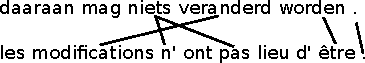
\includegraphics[scale=1]{morphology/al_orig}}
  \hspace{10mm}
  \subfigure[After segmentation]{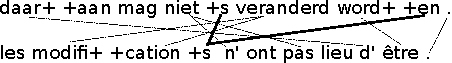
\includegraphics[scale=1]{morphology/al_segm}}
  \caption{Alignment errors increase under segmentation. (English: {\emph Nothing may be changed about that.})}
  \label{fig:m_alignment_error}
\end{figure}

These alignment errors affect both the baseline and clustered systems.
However, the use of a single non-terminal probably allows the baseline system to recover better from bad grammar rules, due to the unrestricted substitution it licenses.
In the clustered cases, on the other hand, the grammars are more constrained by design; there is no mechanism to recover from being constrained in the wrong way, aside from the standard glue rules.

%Comparing only the Hiero-cases, we see that segmentation decreased BLEU ($15.67\to15.57$).
%Segmentation of both languages into morphemes has been shown to have this effect when using phrase-based SMT \citep{Virpioja2007}.
%However, we had expected an even larger decrease, and it might be that segmentation is less harmful in the context of hierarchical phrase-based translation (e.g. Hiero).

A further factor is that BLEU, applied in the standard way, is unforgiving towards partially correct words:
  A word with the correct stem and incorrect inflection gets penalised just the same as a wholly incorrect word.
Such partial improvements should increase the BLEU(m) score, Table~\ref{tbl:m_bleu}:
Segmentation does have this effect, but the unclustered baseline does best by this measure.

Neither the unigram scores nor the percentage of dangling morphemes in the output (i.e. ones that cannot recombine into words) improved under clustering.

On a positive note, however, clustering succeeded in correctly generating words not observed in the training, and for which the other systems failed:

\begin{table}[h]
  \begin{tabular}{llp{0.45\textwidth}}
    Input: & het ivoriaanse model & \multirow{2}{*}{\gloss{the pertaining\_to\_Ivory\_Coast model}} \\
    Reference: & du mod{\`e}le \textbf{ivoirien} \\ \hline
    Baseline:  & du mod{\`e}le \textbf{ivoir\"{i}enne} & incorrect gender \\
    Source clustered: & du \textbf{ivoirien} mod{\`e}le & correct gender, but wrong word order \\
    \phantom{.} \\
    Input: & de antidumpingmaatregelen & \multirow{2}{*}{\gloss{the anti-dumping measures}} \\
    Reference: & des \textbf{mesures antidumping}\\ \hline
    Baseline:  & \textbf{anti mesures dumping}   & correct morphemes, but bad order \\
    Target clustered: & les \textbf{mesures antidumping} & ...although +dumping+ is simply propagated as is from the Dutch input \\
  \end{tabular}
\end{table}

\section{Conclusions and Future Work}
We have presented an approach to using a Hiero-type SCFG to perform translation at the morphology level.
Context-based clustering of morpheme sequences allowed grammar rules to be constrained in way that should limit the formation of non-sensical words.

We found that clustering \textit{per se} succeeded to a large extent.
The clusters we analysed contained strong and clear patterns, learning for example a fine-grained distinction between noun gender in Dutch.

In the context of translation, our approach managed to formulate novel words that were not observed in the training data, and this was a major part of our aim.
On the whole, however, our approach degrades translation quality.

Although our translation results were negative, we would not completely discard the idea of using a SCFG in this way. 
The main problem is that segmenting the data introduces harmful errors into the word alignments.
Bad alignments mean we're screwed from the start. \textit{Thinking out loud. Tone will be fixed later...}

So we have to fix them. 

A further aspect is that translation at the morpheme level is not appropriate in all cases.
We really only want it to be used when confronting rare words or are called upon to create new ones.

A logical next step will be to combine our approach using the back-off grammar work discussed elsewhere in this report.
The idea would be to train a labelled grammar on segmented data (as we have done here) but allow back-off to a grammar trained on the unsegmented data.
This would require sentences to be input to the decoder as lattices, so that there is no hard decision about whether words or morphemes are the best granularity of representation.
This would require modifying the decoding algorithm to recombine morphemes into words when appropriate and score against a language model trained on full words.


%Future possibilities: combine with back-off grammar work, e.g. back-off from a labelled grammar (trained on segmented data) to a Hiero grammar (trained on the unsegmented data).
%express input as a lattice. That way there's no hard decision about whether to use words or morphemes. It would also require changes to decoding: e.g. morphemes will need to be combined into words whenever appropriate and scored against a LM trained on full words.
%
%need to find better solutions to the alignment problems














\chapter{Posterior Regularization}
Posterior regularization is an alternative way of clustering the phrases.
Unlike a Baysian approach where intuitions about the data are expressed through the priors, posterior regularization imposes constraints on posterior distributions of the data.

In this chapter , we will introduce a basic clustering model with EM 
and look at shortcomings of the basic model. This will motivate us for
more complicated posterior regularized models.
\section{Phrase Clustering Model} 
As a brief recap, the clustering problem we are working with
is to label phrases with $K$ induced categories, where
$K$ is picked manually.
Phrases are obtained from bi-text data.
We also look at context
 words before and after
phrases as cues for clustering.
The relationship between phrases, contexts and categories are
represented with a generative model shown in 
Figure \ref{fig:EM}: a phrase picks a 
category and then that category generates the contex for the phrase.

\begin{figure}[h]
  \centering
  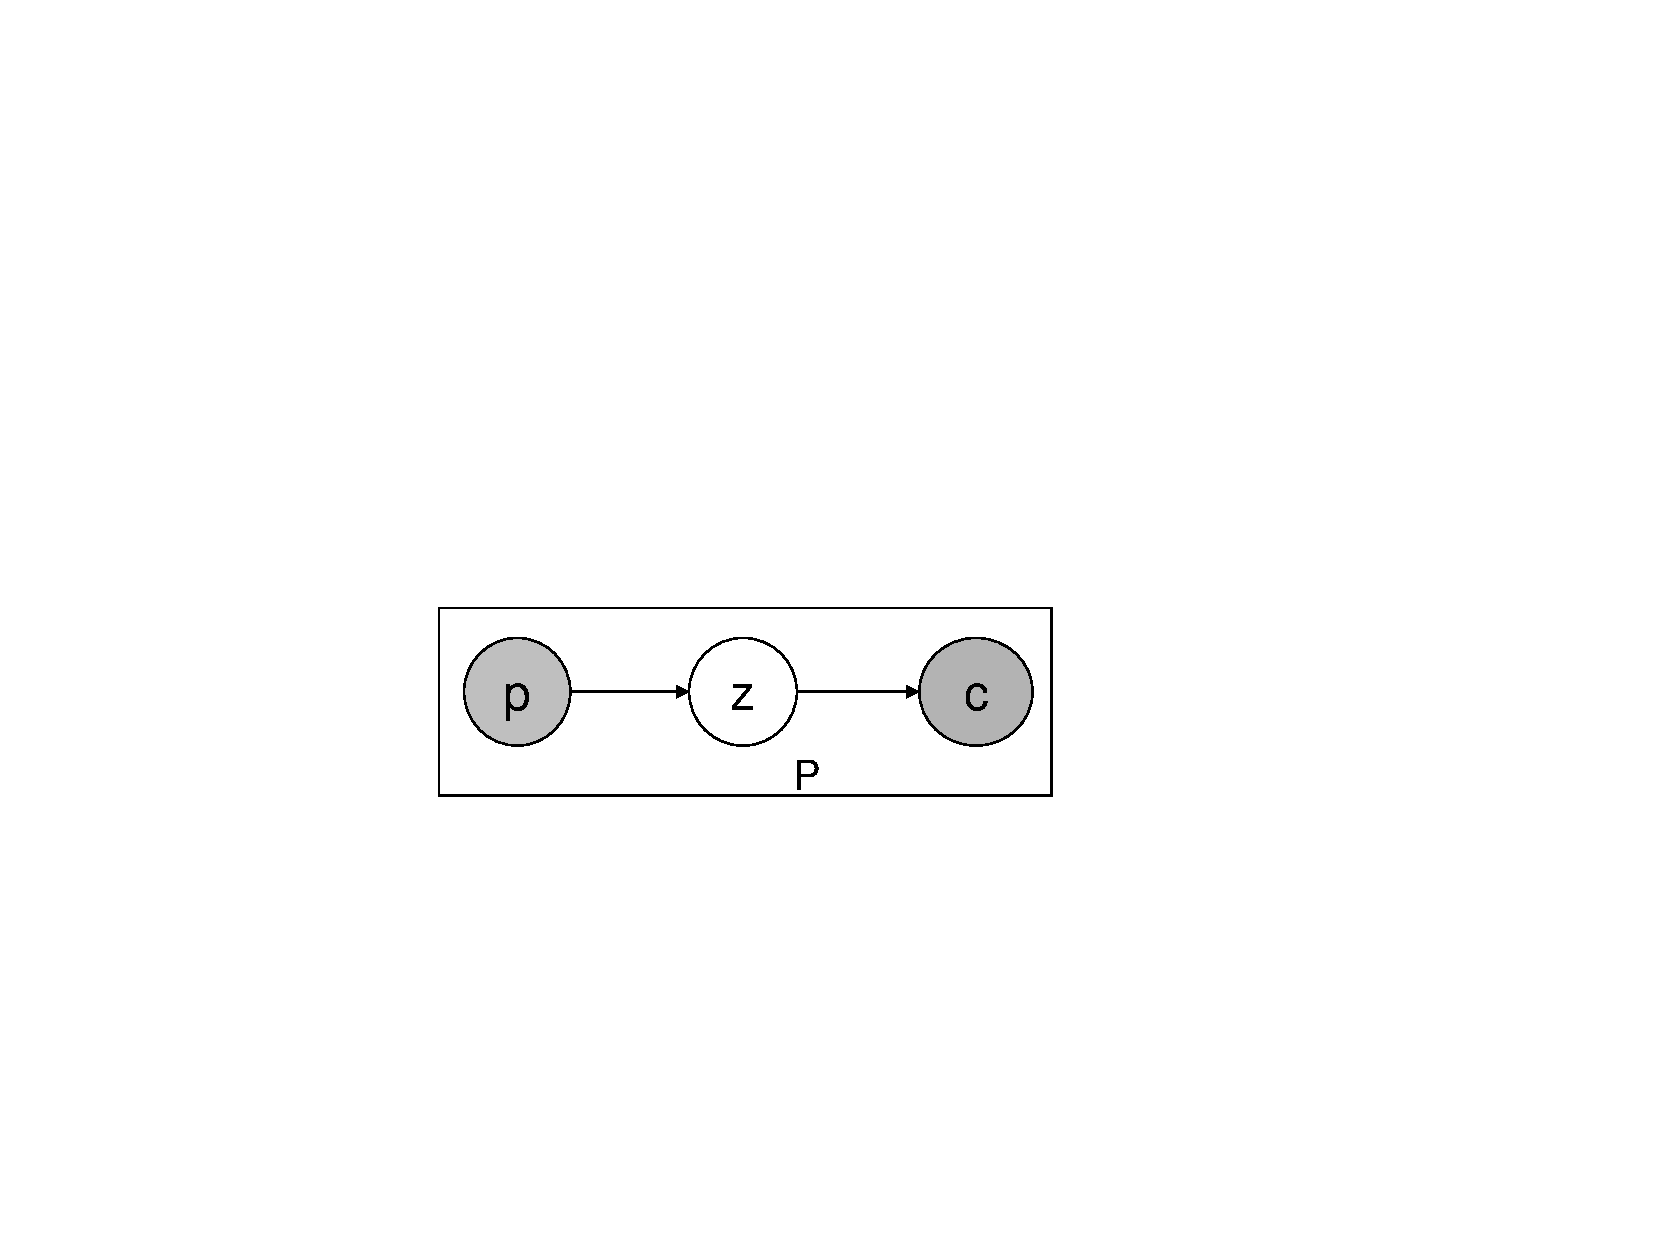
\includegraphics[width=3.0in]{pr-clustering/EMdigram}
  \caption{Basic Phrase Clustering Model}
  \label{fig:EM}
\end{figure}

The joint probability of a category $z$ and a context $\textbf{c}$ 
given a phrase $\textbf{p}$ is
\[
P(z,\textbf{c}|\textbf{p})=P(z|\textbf{p})P(\textbf{c}|z).
\]
$P(z|\textbf{p})$ is distribution of categories given a phrase.
This can be learned from data.
$P(\textbf{c}|z)$ is distribution of context given a category.
Since a context usually contains multiple slots for words, we further
decompose this distribution into independent distributions at
each slot. For example, suppose a context consists of two positions 
before and after the phrase. Denote these words as 
$c_{-2},c_{-1},c_1,c_2$.
Use $P_{-2},P_{-1},P_1,P_2$ to denote distributions of words at each 
position, $P(\textbf{c}|z)$ is decomposed as
\[
P(\textbf{c}|z)=P_{-2}(c_{-2}|z)P_{-1}
(c_{-1}|z)P_1(c_1|z)P_2(c_2|z).
\]
The posterior probability of a category given a phrase
and a context can be computed by normalizing the joint probability:
\[
P(z|\textbf{p},\textbf{c})=\frac{P(z,\textbf{c}|\textbf{p})}
{\sum_{i=1,K}P(i,\textbf{c}|\textbf{p})}.
\]
With the mechanisms to compute the posterior probabilities, we can 
apply EM to learn all the probabilities.
\section{Sparsity Constraints}\label{sec:pr-sparse}
A common linguistic intuition we have about the phrase 
clustering problem is that a phrase should be put into very
few categories, e.g. a verb phrase is unlikely to be used as 
a noun phrase. In other words, the categorization of
a phrase should be sparse.
The generative model we proposed above with EM
allows a phrase to be labelled with many tags. As we observed
from the output, EM is using more categories than we wanted for
each phrase.
Posterior regularization
provides a way to enforce sparsity \citep{ganchev:penn:2009}.
The general idea of posterior regularization is to modify
E-step of EM, so that instead of using posterior distribution
as the $q$ distribution directly, we want to find the nearest
$q$
in a constrained space  as shown in Figure \ref{fig:EMPR}.

\begin{figure}[h]
  \centering
  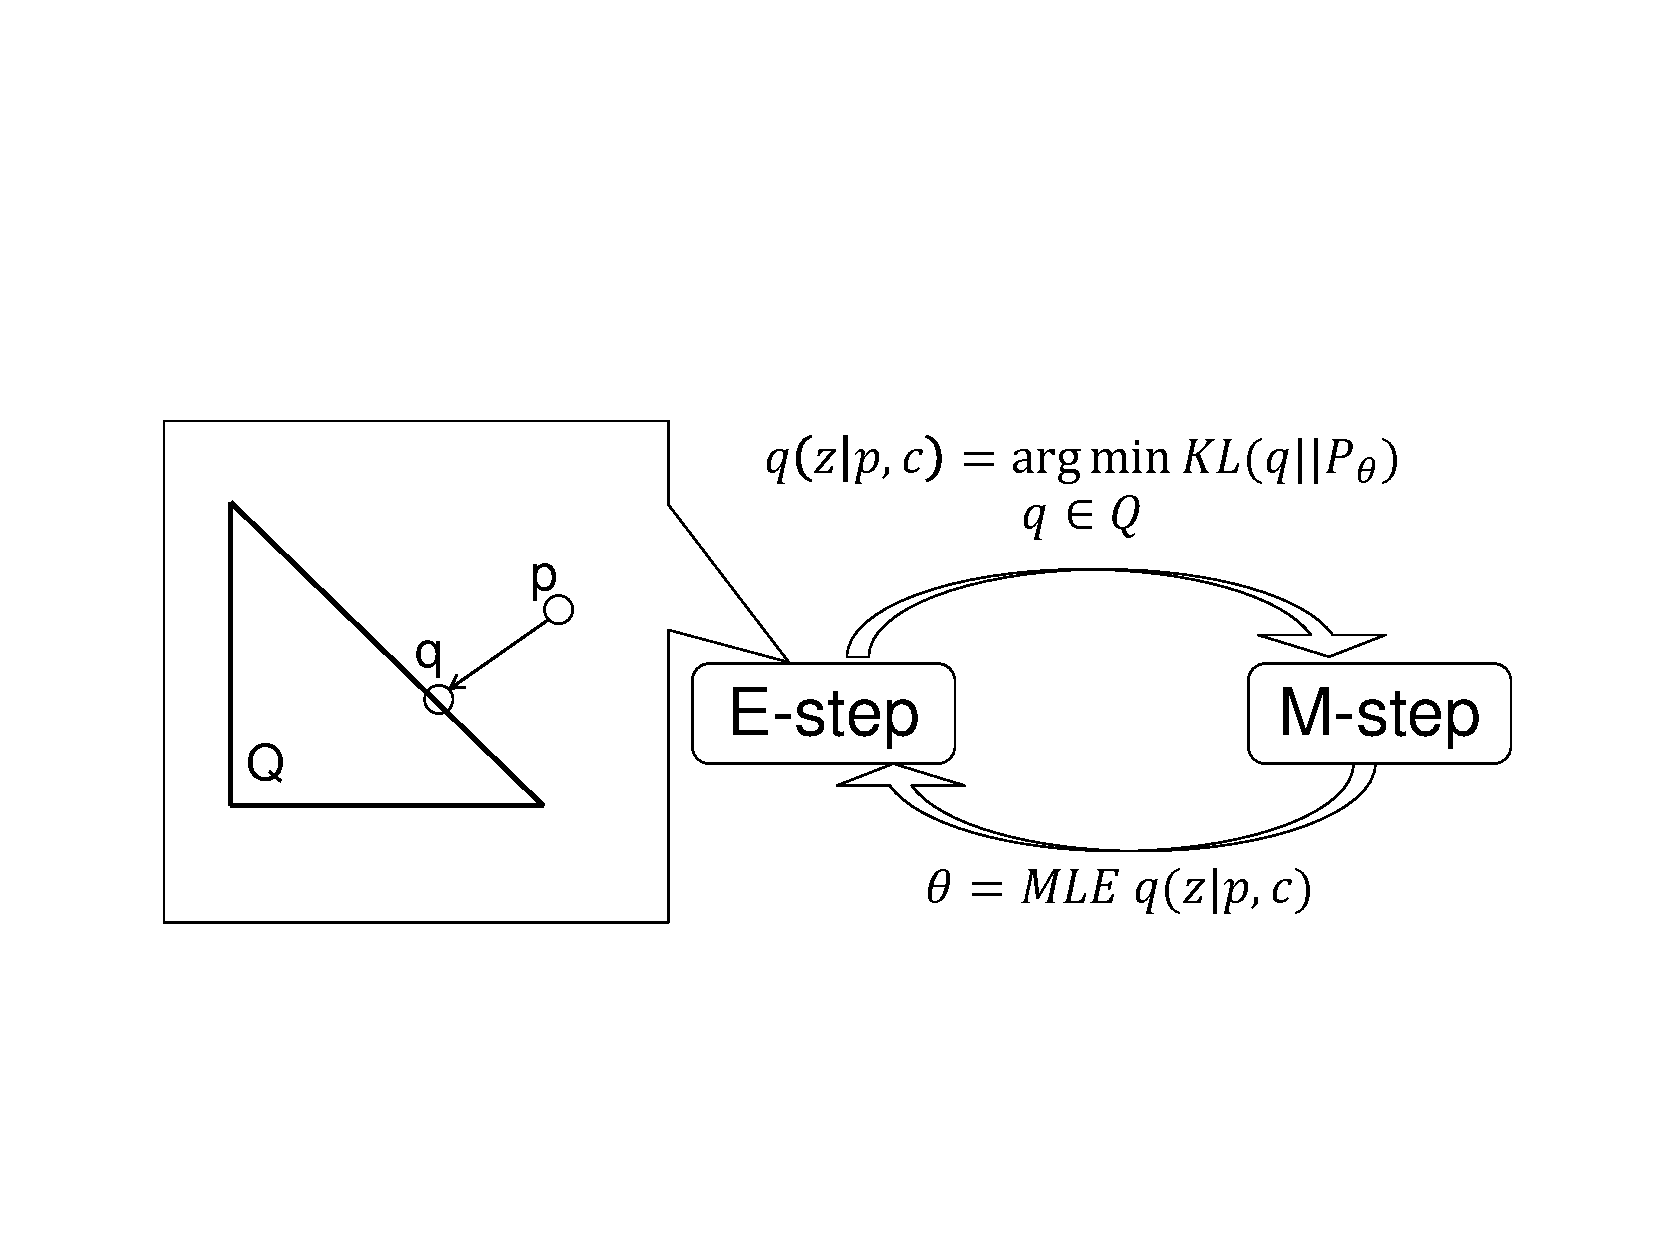
\includegraphics[width=3.5in]{pr-clustering/EMPR}
  \caption{EM with posterior regularization}
  \label{fig:EMPR}
\end{figure}

The constraint we use here is called $l_1/ l_\infty$
regularization in Ganchev's technical report. The notations
we use here largely follows Ganchev's.
In a more mathematical formulation, for each phrase $\textbf{p}$,
we want the quantity 
\[\sum_{z=1}^K \max_i P(z|\textbf{p},\textbf{c}_i) \]
to be small, where $\textbf{c}_i$ is the context
appeared around the $i$th occurrence of phrase $\textbf{p}$
throughout the data. This quantity roughly equals 
the number of categories phrase $\textbf{p}$ uses.
It is minimized to $1$ if and only if
the posterior distributions $P(z|\textbf{p},\textbf{c}_i)$
are the same
for all
occurrences of $\textbf{p}$. That is ,
$\forall i,j$, $P(z|\textbf{p},\textbf{c}_i)=P(z|\textbf{p},\textbf{c}_j)$. 

Define feature functions for $i$th occurrence of phrase $\textbf{p}$
with category $j$,
as a function of category $z$:
\[
\phi_{\textbf{p}ij}(z)=
\begin{cases}
1\text{ if z=j}\\
0\text{ otherwise}
\end{cases}.
\]
For notation simplicity, for
each phrase category pair, 
define variables $c_{\textbf{p}z}$ that will
eventually be $\max_i E_q[\phi_{\textbf{p}iz}]$.
The objective we want to optimize becomes:
\[
\arg\min_{q,c_{\textbf{p}z}} KL(q||P_{\theta}) + 
\sigma \sum_{\textbf{p},z}c_{\textbf{p}z}
\]
\[
\text{ s.t. }\forall \textbf{p},z,
E_q[\phi_{\textbf{p}iz}]\leq c_{\textbf{p}z},
\]
where $\sigma$ is a constant to control
how strongly the soft constraint should
be enforced.
Using Lagrange Multipliers, this objective can
be optimized in its dual form,
for each phrase $\textbf{p}$:
\[
\arg\min_{\lambda\geq 0} \log 
(\sum_{z,i} P_\theta(z|\textbf{p},\textbf{c}_i)
\exp (-\lambda_{\textbf{p}iz}))
\]
\[
\text{ s.t. } \forall \textbf{p},z,
\sum_i \lambda_{\textbf{p}iz}\leq \sigma.
\]
This dual objective can be optimized with projected gradient
descent.
The $q$ distribution we are looking for is then
\[
q_i(z)\propto P_{\theta}(z|\textbf{p},\textbf{c}_i)
\exp(\lambda_{\textbf{p}iz}).
\]
M-step can be performed as usual.
\section{Agreement Models}\label{sec:pr-agree}
Another type of constraint we used is agreement between
different models. We came up with a similar generative
model in the reverse direction to agree with 
as shown in Figure \ref{fig:EMreverse}. We also
took advantage of bi-text data we have and make models
learning from different languages agree with each other.

\begin{figure}[h]
  \centering
  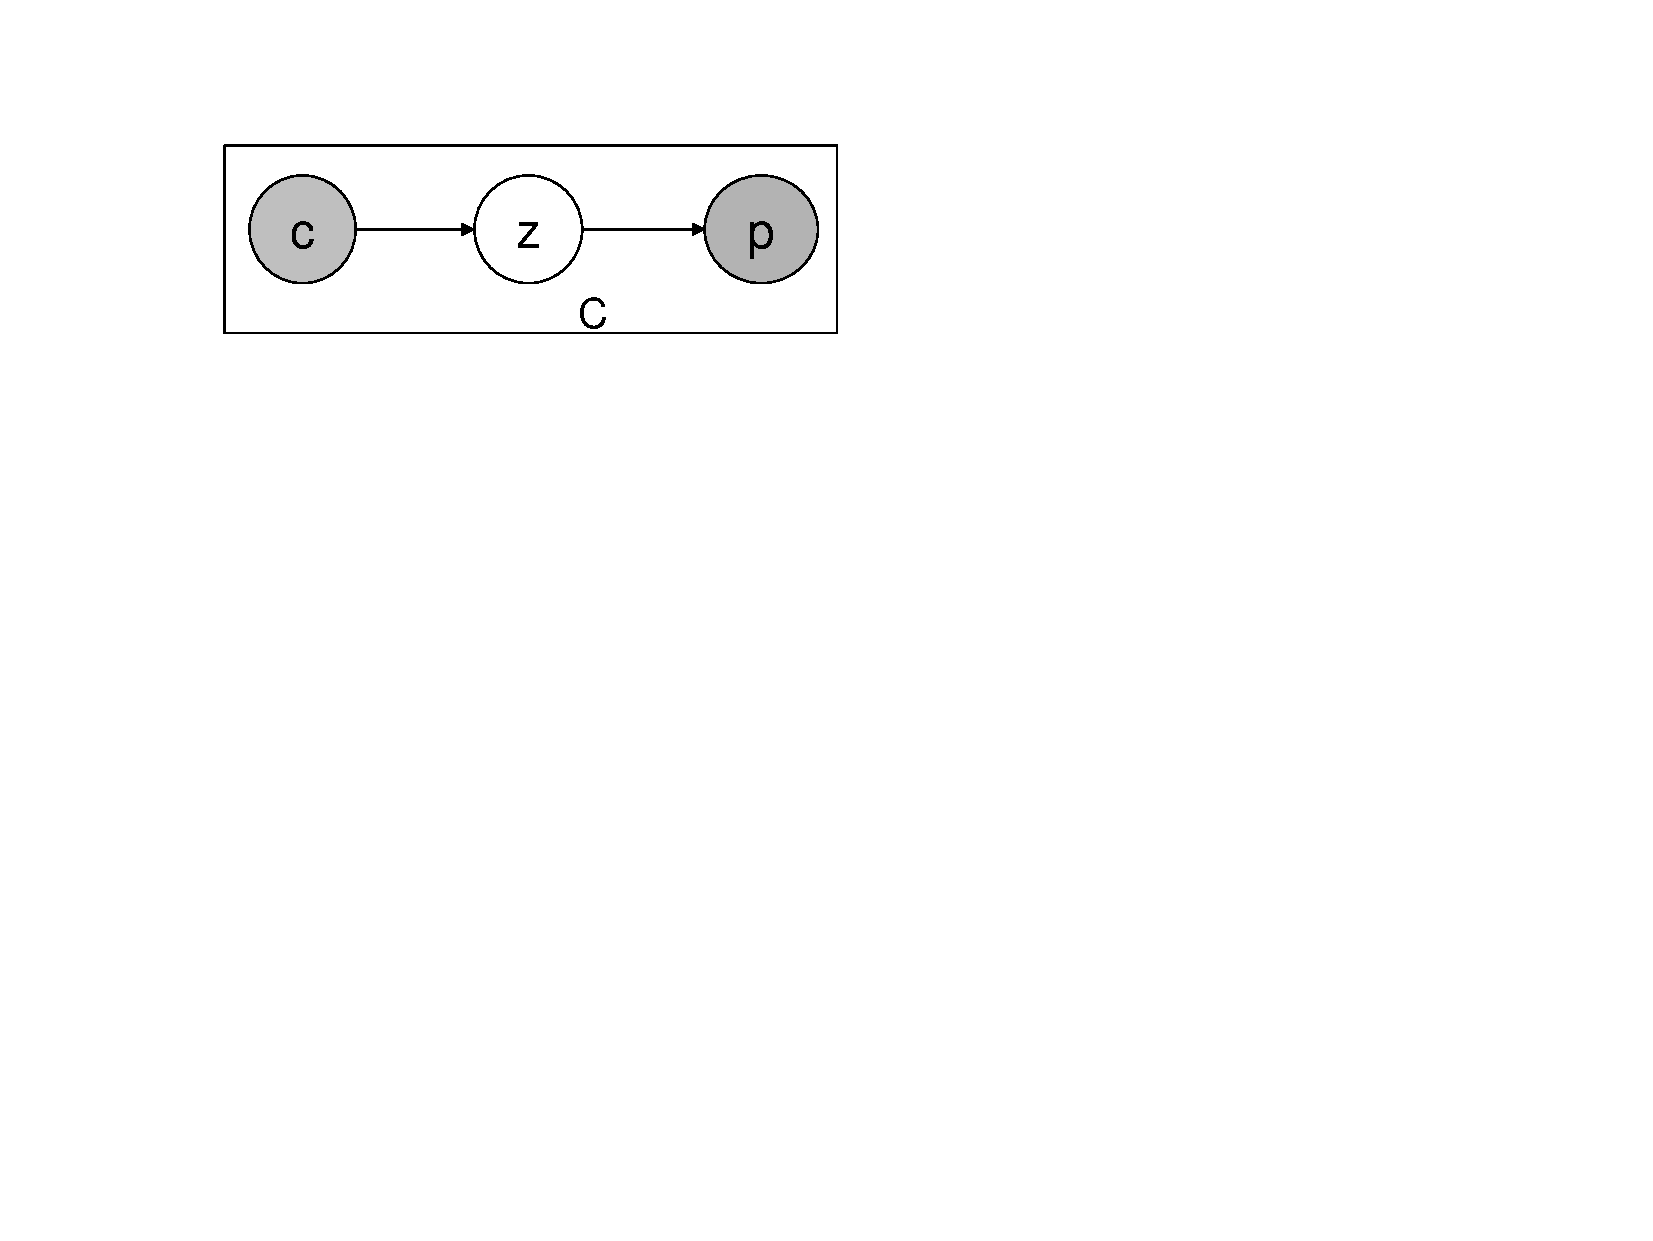
\includegraphics[width=3.0in]{pr-clustering/EMreverse}
  \caption{EM with posterior regularization}
  \label{fig:EMreverse}
\end{figure}

In the reversed model,
the posterior probability of the labelling of
a context $\textbf{c}$ with
phrase $\textbf{p}$ is 
\[
P(z|\textbf{c},\textbf{p})\propto 
P(z|\textbf{c})P(\textbf{p}|z).
\]
Since a phrase contains a variable number of words,
we only look at the first and last word of
a phrase. That is $P(\textbf{p}|z)=P_1(p_1|z)P_n(p_n|z)$,
where $n$ is the length of $\textbf{p}$, $P_1$ and $P_n$
denotes distributions for words in the first and last position
of a phrase given a category.

The implementation of agreement models again ends up making
a small change to E-step. The $q$ distribution for
a phrase $\textbf{p}$ and a context $\textbf{c}$ 
is given by
\[
q(z)=\sqrt{P_{\theta 1}
(z|\textbf{p},\textbf{c})P_{\theta 2}(z|\textbf{p},\textbf{c})},
\]
where $P_{\theta 1}$ and $P_{\theta 2}$ are
posterior distributions for two models.
In M-step, both models should update their parameters with the
same $q$ distribution computed as above.
This modified EM maximizes the objective:
\[
\mathcal{L}_1+
\mathcal{L}_2+
\sum_{\textbf{p},\textbf{c}}
\log\sum_z\sqrt{P_{\theta 1}(z|\textbf{p},\textbf{c})
P_{\theta 2}(z|\textbf{p},\textbf{c})},
\]
where $\mathcal{L}_1$ and $\mathcal{L}_2$
are log-likelihood of
two models.
\section{Experiments}
As a sanity check, we looked at a few examples produced by
the basic model (EM) 
and the posterior regularization (PR) model
with sparsity constraints. Table \ref{tab:EMVSPR}
shows a few examples.

\begin{table}[h]
  \centering
  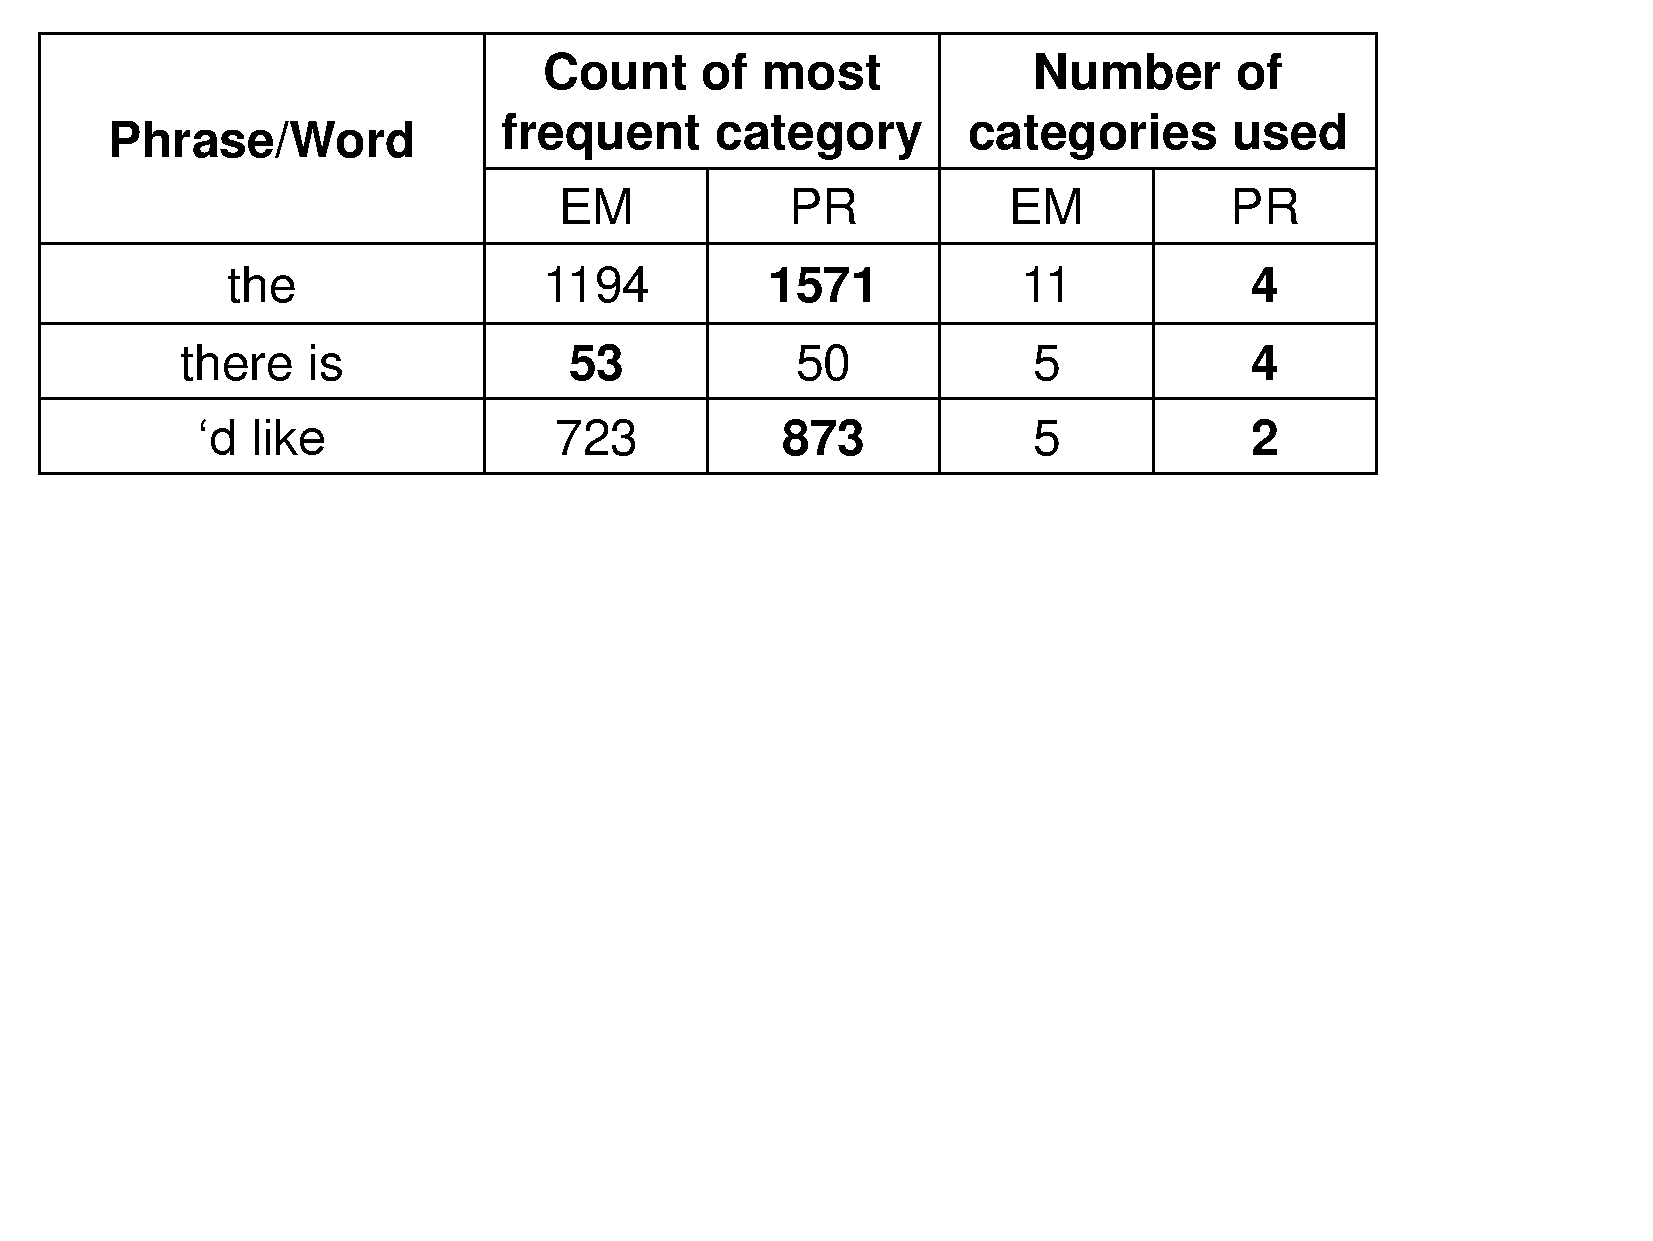
\includegraphics[width=3.5in]{pr-clustering/EMVSPR}
  \caption[A few examples comparing EM and PR]
  {A few examples comparing EM and PR. 
    Count of most frequent category shows how 
    many instances of a phrase are concetrated on 
    the single most frequent tag. 
    Number of categories shows how many categories
    a phrase is labelled with. By experience as mentioned before, 
    we want a phrase to use fewer categories. 
	These numbers are fair indicators of sparsity.
    }
  \label{tab:EMVSPR}
\end{table}

The models are formally evaluated with two kinds
of metrics. We feed the clustering output
through the whole translation pipeline 
to obtain a BLEU score. We also came up 
with an intrinsic evaluation of clustering quality
by comparing against a supervised CFG parser trained on the
tree bank.

We are mainly working on Urdu-English language pair. 
Urdu has very 
different word ordering from English. 
This leaves us room for improvement over
phrase-based systems.
Here in Table \ref{tab:results} 
we show BLEU scores as well as
conditional entropy for each of the models above
on Urdu data. Conditional entropy is computed
as the entropy of ``gold'' labelling given
the predicted clustering. ``Gold'' labelling
distribution
is obtained from Collins parser
trained on Penn Treebank. Since not
all phrases are constituents, we ignored
phrases that don't correspond any constituents.

\begin{table}[h]
  \centering
  \begin{tabular}{ |*{3}{c|} }
    \hline
    model & BLEU & H(Gold$|$Predicted)\\
        \hline
    hiero & 21.1 & 5.77\\
     hiero+POS &  & \\
     SAMT & & \\
     EM & & \\
     PR $\sigma=100$ & & \\
     agree language & & \\
     agree direction & &\\
     non-parametric & & \\
         \hline
  \end{tabular}
    \caption
  {Evaluation of PR models.
	Left column shows BLEU scores
	through the translation pipeline.
	Right columns shows conditional entropy
	of the 
    }
  \label{tab:results}
\end{table}

In Table \ref{tab:results}, hiero is hierachical phrase-based
model with 1 category in all of its SCFG rules. Hiero+POS
is hiero with all words labelled with their POS tags.
SAMT is a syntax based system with a supervised
parser trained on Treebank. EM is the first model mentioned
in the beginning of this chapter. PR $\sigma=100$ is 
posterior regularization model with sparsity constraint
explained in Section \ref{sec:pr-sparse}.
$\sigma$ is the constant controls strongness of the constraint.
Agree language and agree direction are models with agreement 
constraints mentioned in Section \ref{sec:pr-agree}. Non-parametric
is non-parametric model introduced in the previous chapter.

\section{Conclusion}

\chapter{Training}

An integral part of constructing a state-of-the-art machine translation system is the training procedure. The goal of training is to optimize the model parameters to maximize translation quality on some metric, where the parameters are the weights associated with the features we use in our model, and the metric is BLEU. 

The most common approach to training is Minimum Error Rate Training (MERT), which tunes the parameters to minimize error according to an arbitrary error function. Thus, in our case this is equivalent to saying that it maximizes the 1-best translation under the BLEU metric. MERT is a log-linear model which allows us to combine different features in order to find the best target translation $e*$ for a input source $f$:
$$e* = \arg\max e p(e|f) = argmax_e \sum_{k=1}^K w_kh_k(e,f)$$

where $h_k(e,f)$ is a feature associated with the translation of $f$ to $e$, and $w$ is the weight associated with that feature. Unfortunately, MERT has been empirically unable to extend beyond optimization of a handful of features, thus necessecitating dense features. Theses features typically include:

\begin{itemize}
\item rule relative frequency $P(e|f)$
\item target $n$-gram language model $P(e)$
\item `pass-through' penalty when passing a source word to the target side untranslated
\item lexical translation probabilities $P_{lex}(\overline{e}|\overline{f})$ and $P_{lex}(\overline{f}|\overline{e})$
\item count of the number of times that arity-0,1, or 2 SCFG rules were used 
\item count of the total number of rules used
\item source word penalty
\item target word penalty
\item count of the number of times the glue rule is used 
\end{itemize} 

However, after the creation of the refined grammars which have been described in the previous sections, we have additional information available to us which we would like to leverage in order to improve translational performance. The way in which we would like to utilize this informaiton is by extracting it as features for our model. For instance, some features of particular instance may be:

\section{Feature Extraction}
There are a number potentially useful features we could extract from the refined grammars, such as:
\begin{itemize}
\item Source Syntactic Features
\item Target Syntactic Features
\item Source Context Features
\item OOV
\item Glue Rule
\item Morphology
\end{itemize}


\subsection{Source Syntactic Features}

Recent work with syntax-based systems which parse the source side with a previously trained supervised parser has shown that utilizing syntactic patterns can lead to substantial improvements. Such patterns can be especially useful in capturing long-range reordering patterns, and other high-level phenomena that we are otherwise unable to leverage. Figure~\ref{fig:synt_feat1} shows an example syntactic pattern, which captures the application of rule $X_{12}$ expanding to $X_{17}X_{25}$. Although this rule may not be particularly interesting, as the translation stays monotonic. 

\begin{figure}[h]
	\centering
		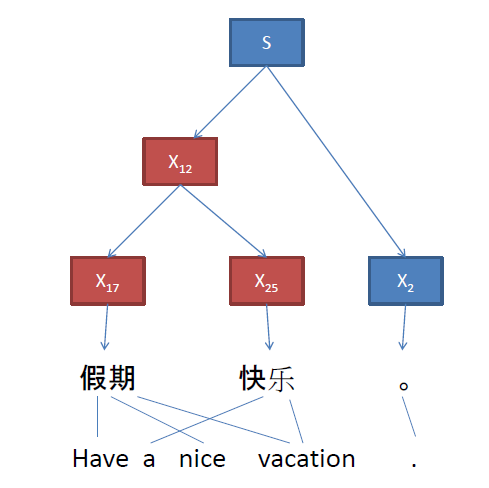
\includegraphics[scale=0.5]{training_img_files/synt_feat1.PNG}
	\caption{Syntactic Feature}
	\label{fig:synt_feat1}
\end{figure}

A more interesting example is presented in Figure~\ref{fig:synt_feat2}, where we can observe a large reodering taking place as $X_1$ expands to $X_6X_19$ and the latter moves to the left of the former.

\begin{figure}[h]
	\centering
		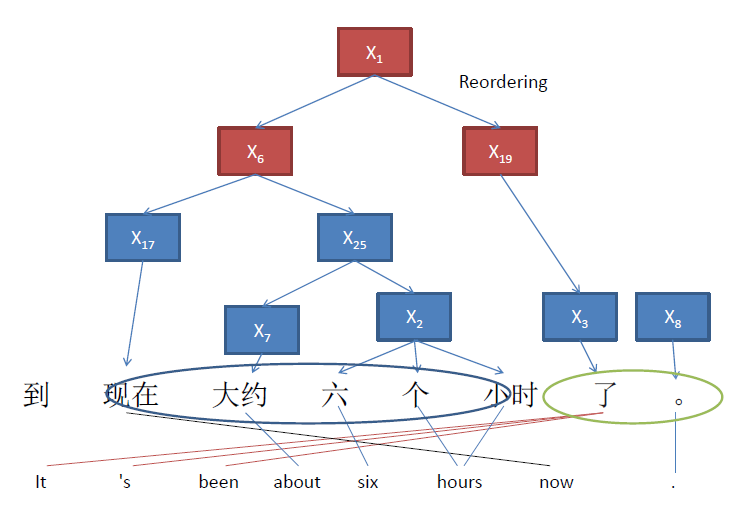
\includegraphics[scale=0.5]{training_img_files/synt_feat2.PNG}
	\caption{Syntactic Reordering Feature}
	\label{fig:synt_feat2}
\end{figure}


\subsection{OOV}
Although we will always encounter Out-of-Vocabulary terms, we may be able to utilize the finer-grained categories to capture syntactic distribution patterns associated with each category to learn how to process the OOV terms. This may be particularly useful for numbers, nouns such as Proper names, or certain adjectives, which tend to cluster togther, as shown in Figure~\ref{fig:oov_feat}.

\begin{figure}[h]
	\centering
		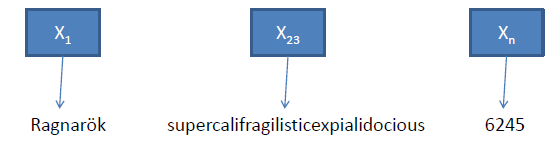
\includegraphics[scale=0.5]{training_img_files/oov_feat.PNG}
	\caption{OOV Feature}
	\label{fig:oov_feat}
\end{figure}

\subsection{Glue Rule}
In our current system, we have one dense feature for all Glue rule applications, however, there are in fact two seperate applications which we would like to distinguish. The first occurs when a top-level $S$ node expands to one of the $X_n$ categories in the grammar, as shown in Figure~\ref{fig:glu_feat}. The second occurs when an $S$ expands to another $S$ and one of the $X_n$ categories, as in Figure~\ref{glu_feat2}. Both of these features attempt to capture the high-level derivation structure of a sentence. 

\begin{figure}[h]
	\centering
		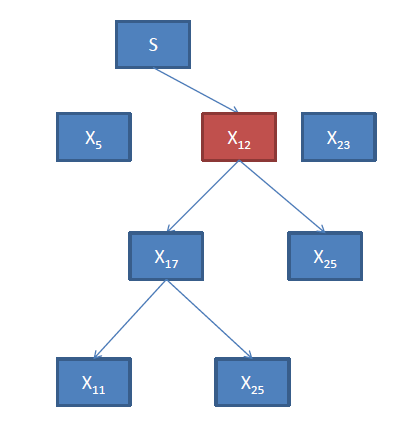
\includegraphics[scale=0.5]{training_img_files/glu_feat.PNG}
	\caption{Glue Rule Expansion Feature}
	\label{fig:glu_feat}
\end{figure}


\begin{figure}[h]
	\centering
		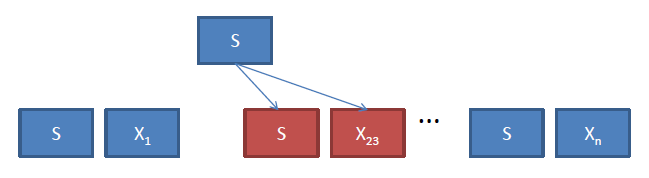
\includegraphics[scale=0.5]{training_img_files/glu_feat2.PNG}
	\caption{Glue Rule Combination Feature}
	\label{fig:glu_feat2}
\end{figure}

\subsection{Backoff}
Given that we have achieved significant gains from incorporating the hierarchical-bacoff feature as a dense feature, it may also be useful to add a sparser version in additional to or in place of the feature we currently use, of the form shown in Figure~\ref{fig:back_feat}.


\begin{figure}[h]
	\centering
		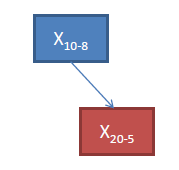
\includegraphics[scale=0.5]{training_img_files/back_feat.PNG}
	\caption{Backoff Feature}
	\label{fig:back_feat}
\end{figure}

\section{Training Algorithms}

As we are interested in incorporating numerous features into our model to directly help translation, we want to perform discriminative training. Given the fact that MERT is unable to optimize the sparse features we are interested in, in this workshop we investigated two alternative methods which allow us to train a model with a high dimensional feature space. The two approaches were the Margin Infused Relaxed Algorithm (MIRA) and Expected BLEU. All three optimization algorithms perform inference over the hypergraph, but as Table~\ref{tab:comp} shows, they are performing in quite different ways. MERT aims to optimize parameters to maximize the 1-best BLEU, or alternatively to minimize the error, by constructing a piece-wise linear error surface from the entire tuning set and performing a line search in order to find the appropriate weights. The primary limitation of this, which is responsible for its inability to scale, is the unknown diretion of the line search. When done in a handful of dimensions, random directions work relatively well, however, as we increase the feature space this becaomes a severe problem. 

Expected BLEU training, explained in detail in Section~\ref{sec:exp_bleu} is a probabilistic method which can be seen as an attempt to address some of these shortcomings. If instead of maximizing the 1-best hypothesis, as we do with MERT, we try to maximize the expected BLEU over all the hypotheses, we create a continuous, and therefore differentiable function for optimization which allows us to use gradient-based methods, such as L-BFGS. 

MIRA training, on the other hand, is a large-margin based training method, which attempts to miminimze the loss augmented score of hypotheses against some reference translation in an online fashion. In order to do so, we need to solve a Quadratic optimization problem with linear constraints, which can be handled by a technique such as Sequential Minimal Optimization (SMO). The foremost downside of this approach is the approximation of the reference that needs to take place for the training to proceed. Since the MT grammar may not contain the necessary rules to produce the correct reference translation, therefore making the translation unreachable, we need to rely on an approximation of the reference. Previous work has explred various approaches for this, such as updating toward the model 1-best, or oracle 1-best. Another possibility is that there may be multiple derivations which lead to the same translation, therefore creating ambiguity regarding which rules, and features should be updated towards. We will expand on this in Section~\ref{sec:mira}.

\begin{table*}[htb]
	\centering
		\begin{tabular}{|c|c|c|c|} 
			& MERT & MIRA & Expected BLEU \\ \hline
			Type & 1-best & Margin-based & Probabilistic \\ \hline
			Objective & Minimize error & Minimize loss augmented score & Minimize expected error \\ \hline
			Optimization & Line search & QP & Gradient Based \\ \hline
			Limitations & Direction of search unknown & Approximation of reference & Approximate expectation \\ \hline
		\end{tabular}
	\caption{Training Comparison}
	\label{tab:TrainingComparison}
\end{table*}

\section{Margin Infused Relaxed Algorithm}
\label{sec:mira}

MIRA was first introduced in 2003 by Crammer and Singer for the multi-class classification problem as a perceptron like algorithm, with the additional of a classifcation margin to reduce generalization error. This was later expanded by Taskar to structured value prediction problems, such as dependency parsing. It was notably applied to machine translation by Watanabe, and then Chiang, on whose work we build here.

\subsection{Learning Algorithm}
The basic online learning algorithm proceeds as in Algorithm X. We go through the data for $n$ iterations, and during each iteration we go through all our data points and update the weight vector after each example. We then use the new weight vector to process the next example, and so on, until we reach some convergence criteria. After convergence, we average over the weight vectors to produce a final weight vector which we can use to process new examples. The averaging of the weight vector is done to reduce overfitting, and has proved effective in previous applications. 

When performing inference over the hypergraph, each edge in the hypergraph corresponds to a partial translation and has associated with it a decomposable score $s$:
$$s(edge_i) = w*f(edge_i)$$
which is comprised of the features on that edge and the current weight vector. These can then be added together to produce the score associated with a specific hypothesis translation:
$$\sum_{edge \in derivation} s(edge)= S(e) $$

We also compute a decomposable loss at each edge,which is the approximate BLEU score of the partial hypothesis on the edge. 
What we want is to learn $w$ such that the correct output translation is given a higher score than the incorrect ones. The MIRA update does this optimization by keeping the norm of the change of the weights as small as possible
$$ min ||w_{i+1} - w_i||$$
subject to the margin constraints, which take the following form:
$$ s(x,y) - s(x,z) \geq Loss(y,z), \forall{z} \in label(x)$$

Essentially, these margin constraints force us to create a margin between the correct instance y, and the incorrect instance z which is at least as large as the Loss of z.




\subsection{Oracle Extraction}
In multi-class classification, we can form the constraint set by looking at all the possible labels of x, however, in structured prediction, this becomes infeasible. Thus, in practice previous work has resorted to approximating the constraint set by performing k-best extraction over the trees in dependency parsing, or translations in MT, using only these top $k$ labels as constraints in training. This leads to the modified training algorithm of k-best MIRA, described in Algorithm Y. 

For MT, recent work has shown significant improvements from obtaining three different sets of k-best lists. The first is the model k-best
$$w*f(e) $$
 the second is the model+BLEU, also referred to as the oracle or hope hypothesis The first translation in this k-best set is the oracle translation toward which we update:
 $$w*f(e) + BLEU $$
 and the third is model-BLEU, or the feat hypothesis:
 $$w*f(e) - BLEU $$
 

The impetus behind updating toward towards a combination of the model and BLEU as the oracle translation is that some translations may have an excellent BLEU score, but a distant model score from the area in which most good translation reside, and parroting Voltaire, we do not want to the perfect to be the enemy of the good. 
 
The reasoning behind the third set of k-best lists is that the constraints we care most about for learning are the ones where our system believes the hypothesis is a good one, and thus assigns it a high score, while the BLEU score is poor, thus proving in fact to be a poor translation. 

\subsection{Online Updating}
In order to efficiently train an online learning, significant modifications were necessary to our existing parallelization framework. As updating the weight vector after each example may be inadvisable since the weights could suffer significant jumping around, we could perform mini-batch updating, where weights are only updated after a certain amount of examples have been processed. An alternative which is similar in spirit is to run several learners in parallel, and have them share their k-best hypotheses sets between themselves, in order for each learner to incorporate more information at each update. Figure ~\ref{fig:update1} presents three learners receiving a sentence in parallel. Each learner has its own MIRA trainer and decoder, with its own feature weight vector. In Figure ~\ref{fig:update2} we see Learner 1 completing its decoding of the sentence with its current weight vector, and generating the three k-best lists as described above. It then uses these to update its weights for decoding the next sentence. In Figure ~\ref{fig:update3} we see that both Learner 1 and 2 have completed decoding and generate their respective k-best lists, and these are passed to Learner 3 in order for it to incorporate them, as well as it's own set of k-best lists, when it updates its weight vector.

\begin{figure}[h]
	\centering
		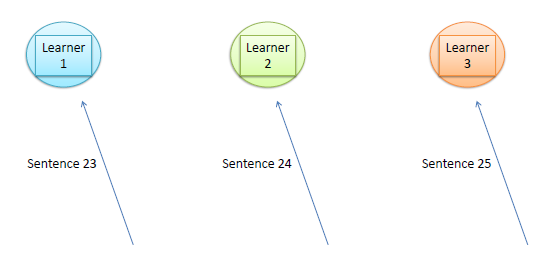
\includegraphics[scale=0.5]{training_img_files/update1.PNG}
	\caption{Online Udpating 1)}
	\label{fig:update1}
\end{figure}


\begin{figure}[h]
	\centering
		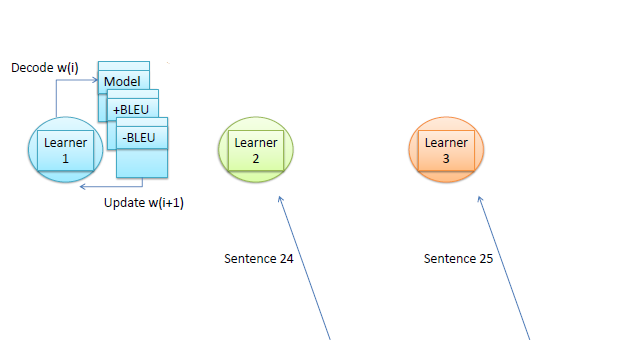
\includegraphics[scale=0.5]{training_img_files/update2.PNG}
	\caption{Online Udpating 2)}
	\label{fig:update2}
\end{figure}


\begin{figure}[h]
	\centering
		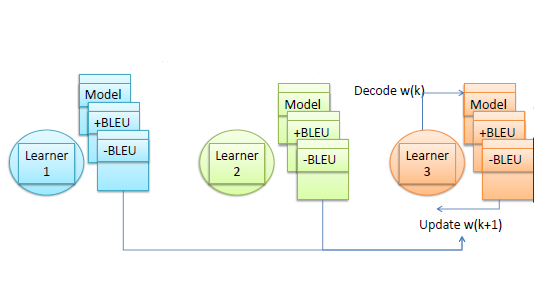
\includegraphics[scale=0.5]{training_img_files/update3.PNG}
	\caption{Online Udpating 3)}
	\label{fig:update3}
\end{figure}

\section{Expected BLEU}
\label{sec:exp_bleu
}
\section{Accomplishments}
During the workshop, we succeeded in completely implementing MIRA and Expected BLEU training in Joshua and cdec, two state-of-the-art open source decoders. This includes the ability to extract oracles from the lattices, as well as the online updating parallelization architecture. Due to a lack of time and resources, we were unfortunatley unable to run the full suite of experiments which we had hoped for, but we leave these as immediate future work.

\section{Future Work}
The first set of experiments concerns a standardized comparison of MIRA and Expected BLEU training, using as-close-as-possible simliar grammas, features, and data sets. To the best of our knowledge, a systematic comparison of these two popular training algorihtms has not been performed, and would be of benefit to the community. 

Second, we are interested in the language invariability of the parameters, number of iterations, and so forth for these algorthims. 




\bibliographystyle{apalike}
\bibliography{biblio}

\printindex

\end{document}
